% E-Sahulat technical report. Build: cd report && tectonic technical_report.tex
% Numbers come from generated/data.tex, written by make_report_data.py from the notebook's outputs.
\documentclass[11pt,a4paper]{article}

% ------------------------------------------------------------------ fonts (XeTeX / Tectonic)
\usepackage{fontspec}
\setmainfont{texgyrepagella}[Extension=.otf, UprightFont=*-regular, BoldFont=*-bold, ItalicFont=*-italic, BoldItalicFont=*-bolditalic]
\setsansfont{texgyreheros}[Extension=.otf, UprightFont=*-regular, BoldFont=*-bold, ItalicFont=*-italic, BoldItalicFont=*-bolditalic, Scale=0.95]
\setmonofont{lmmono10-regular}[Extension=.otf, Scale=0.95]
\newfontfamily\urdufont{Amiri-Regular.ttf}[Script=Arabic, Language=Urdu, Scale=1.05]
\TeXXeTstate=1
\newcommand{\ur}[1]{{\urdufont\beginR #1\endR}}

% ------------------------------------------------------------------ layout and packages
\usepackage[margin=2.3cm, headheight=14pt]{geometry}
\usepackage{amsmath, amssymb}
\usepackage{graphicx}
\usepackage{booktabs, tabularx, array, multirow, colortbl}
\renewcommand{\tabularxcolumn}[1]{>{\raggedright\arraybackslash}p{#1}}
\usepackage{xcolor}
\usepackage{float}
\usepackage{caption, subcaption}
\usepackage{enumitem}
\usepackage{fancyhdr}
\usepackage{titlesec}
\usepackage[most]{tcolorbox}
\usepackage{tikz}
\usetikzlibrary{arrows.meta, positioning, shapes.geometric, shapes.misc, shapes.symbols, fit, backgrounds, calc, decorations.pathreplacing}
\usepackage{pgfplots}
\pgfplotsset{compat=1.18}
\usepackage[hidelinks]{hyperref}

\setlist{itemsep=2pt, topsep=4pt}
\captionsetup{font=small, labelfont={bf,sf}, labelsep=period}
\setlength{\parskip}{4pt}
\setlength{\parindent}{0pt}

% palette shared with the web app (DESIGN.md)
\definecolor{esgreen}{HTML}{1D4A37}
\definecolor{esgreendeep}{HTML}{153728}
\definecolor{esseries}{HTML}{1F8A5F}
\definecolor{esblue}{HTML}{2F6FC4}
\definecolor{esrose}{HTML}{C25E8A}
\definecolor{esviolet}{HTML}{5A3EA8}
\definecolor{esochre}{HTML}{8A5A00}
\definecolor{esred}{HTML}{B3261E}
\definecolor{espaper}{HTML}{F3F3F0}
\definecolor{essheet}{HTML}{FBFBF8}
\definecolor{esink}{HTML}{1B1B1F}
\definecolor{esink2}{HTML}{45454C}
\definecolor{esrule}{HTML}{DCDBD4}

\titleformat{\section}{\sffamily\Large\bfseries\color{esgreen}}{\thesection}{0.7em}{}
\titleformat{\subsection}{\sffamily\large\bfseries\color{esink}}{\thesubsection}{0.6em}{}
\titleformat{\subsubsection}{\sffamily\normalsize\bfseries\color{esink2}}{\thesubsubsection}{0.6em}{}
\titlespacing*{\section}{0pt}{18pt}{8pt}

\pagestyle{fancy}
\fancyhf{}
\fancyhead[L]{\sffamily\small\color{esink2}E-Sahulat AI \textbullet{} Technical report}
\fancyhead[R]{\sffamily\small\color{esink2}\leftmark}
\fancyfoot[C]{\sffamily\small\thepage}
\renewcommand{\headrulewidth}{0.4pt}
\renewcommand{\headrule}{{\color{esrule}\hrule width\headwidth height\headrulewidth}}
\renewcommand{\sectionmark}[1]{\markboth{#1}{}}

% callout boxes
\newtcolorbox{keybox}[1][]{enhanced, colback=essheet, colframe=esgreen, boxrule=0.6pt, arc=2pt, left=8pt, right=8pt, top=6pt, bottom=6pt,
  fonttitle=\sffamily\bfseries\small, coltitle=white, colbacktitle=esgreen, title={#1}}
\newtcolorbox{notebox}[1][]{enhanced, colback=espaper, colframe=esrule, boxrule=0.5pt, arc=2pt, left=8pt, right=8pt, top=5pt, bottom=5pt,
  fonttitle=\sffamily\bfseries\small, coltitle=esink, colbacktitle=esrule, title={#1}}

% KPI tile
\newcommand{\kpi}[3]{%
  \begin{tikzpicture}
    \node[draw=esrule, fill=essheet, rounded corners=2pt, minimum width=3.7cm, minimum height=2.25cm, inner sep=5pt] (b) {};
    \node[anchor=north west, font=\sffamily\scriptsize\color{esink2}, text width=3.4cm] at ($(b.north west)+(4pt,-4pt)$) {#1};
    \node[font=\sffamily\bfseries\LARGE\color{esgreen}] at ($(b.center)+(0,-2pt)$) {#2};
    \node[anchor=south west, font=\sffamily\tiny\color{esink2}, text width=3.4cm] at ($(b.south west)+(4pt,4pt)$) {#3};
  \end{tikzpicture}}

% stamp, as drawn in the app
\newcommand{\stamp}[2]{\tikz[baseline=-0.6ex]{\node[draw=#1, line width=1.1pt, rounded corners=3pt, inner sep=3pt, rotate=-4,
  font=\sffamily\bfseries\scriptsize, text=#1] {\uppercase{#2}};}}

% plot helper: \addplotcoords{options}{\macro} expands the macro before pgfplots reads it
\def\addplotcoords#1#2{\expandafter\addplotcoordsi\expandafter{#2}{#1}}
\def\addplotcoordsi#1#2{\addplot[#2] coordinates {#1};}

\pgfplotsset{
  esaxis/.style={axis line style={esrule}, tick style={esrule}, major grid style={esrule!70}, ymajorgrids=false, xmajorgrids=false,
    tick label style={font=\sffamily\scriptsize}, label style={font=\sffamily\small}, legend style={font=\sffamily\scriptsize, draw=none, fill=none},
    every axis title/.style={font=\sffamily\small\bfseries, at={(0.5,1)}, above}},
}

% generated by report/make_report_data.py; do not edit
\newcommand{\PipelineVersion}{d089d88a44a2}
\newcommand{\StubVersion}{841339e5e722}
\newcommand{\DenseModel}{intfloat/multilingual-e5-base}
\newcommand{\DenseBackend}{neural}
\newcommand{\FinalMethod}{BM25-norm+lex}
\newcommand{\TauDense}{0.8231}
\newcommand{\TauCov}{0.0}
\newcommand{\TauUnknown}{2}
\newcommand{\StubTauDense}{0.6003}
\def\SplitEn{(Dev,53) (Test,13) (Brief,4) (Blind,22)}
\def\SplitUr{(Dev,40) (Test,7) (Brief,4) (Blind,11)}
\def\SplitRoman{(Dev,46) (Test,40) (Brief,4) (Blind,14)}
\newcommand{\NDev}{139}
\newcommand{\NTest}{60}
\newcommand{\NBrief}{12}
\newcommand{\NBlind}{47}
\newcommand{\NQueriesAll}{258}
\newcommand{\NDevOfficial}{90}
\newcommand{\NDevTeam}{49}
\def\RetMethods{BM25-raw,CharNgram-TFIDF,BM25-norm+lex,BM25-norm+lex+bi,Dense,Dense-bi,Dense-bi+lex,Hybrid,Hybrid+lex,BM25-norm+lex+bi+rerank,Hybrid+lex+rerank}
\def\RetDevRecall{(0.57,BM25-raw) (0.57,CharNgram-TFIDF) (1.0,BM25-norm+lex) (1.0,BM25-norm+lex+bi) (0.935,Dense) (0.944,Dense-bi) (1.0,Dense-bi+lex) (0.972,Hybrid) (1.0,Hybrid+lex) (1.0,BM25-norm+lex+bi+rerank) (1.0,Hybrid+lex+rerank)}
\def\RetDevMRR{(0.478,BM25-raw) (0.496,CharNgram-TFIDF) (1.0,BM25-norm+lex) (0.986,BM25-norm+lex+bi) (0.829,Dense) (0.847,Dense-bi) (0.92,Dense-bi+lex) (0.936,Hybrid) (0.995,Hybrid+lex) (1.0,BM25-norm+lex+bi+rerank) (0.995,Hybrid+lex+rerank)}
\newcommand{\RetDevN}{107}
\def\RetTestRecall{(0.875,BM25-raw) (0.85,CharNgram-TFIDF) (1.0,BM25-norm+lex) (1.0,BM25-norm+lex+bi) (0.875,Dense) (0.925,Dense-bi) (1.0,Dense-bi+lex) (0.975,Hybrid) (1.0,Hybrid+lex) (1.0,BM25-norm+lex+bi+rerank) (1.0,Hybrid+lex+rerank)}
\def\RetTestMRR{(0.769,BM25-raw) (0.761,CharNgram-TFIDF) (0.958,BM25-norm+lex) (0.971,BM25-norm+lex+bi) (0.8,Dense) (0.798,Dense-bi) (0.946,Dense-bi+lex) (0.905,Hybrid) (0.988,Hybrid+lex) (0.971,BM25-norm+lex+bi+rerank) (0.988,Hybrid+lex+rerank)}
\newcommand{\RetTestN}{40}
\newcommand{\BaseRecall}{0.875}
\newcommand{\BaseMRR}{0.769}
\newcommand{\FinalRecall}{1.000}
\newcommand{\FinalMRR}{0.958}
\newcommand{\DenseRecall}{0.875}
\newcommand{\HybridLexMRR}{0.988}
\def\BlindLabels{Decision acc.,Answer recall,False answers,Citation support,Recall@5,MRR@5}
\def\BlindBase{(Decision acc.,0.766) (Answer recall,0.909) (False answers,0.571) (Citation support,0.533) (Recall@5,0.939) (MRR@5,0.677)}
\def\BlindStub{(Decision acc.,0.723) (Answer recall,0.848) (False answers,0.571) (Citation support,0.607) (Recall@5,0.848) (MRR@5,0.672)}
\def\BlindEfive{(Decision acc.,0.723) (Answer recall,0.818) (False answers,0.429) (Citation support,0.556) (Recall@5,0.848) (MRR@5,0.672)}
\newcommand{\BlindBaseAcc}{76.6\%}
\newcommand{\BlindStubAcc}{72.3\%}
\newcommand{\BlindEfiveAcc}{72.3\%}
\newcommand{\BlindNAcc}{47}
\newcommand{\BlindBaseFalse}{57.1\%}
\newcommand{\BlindStubFalse}{57.1\%}
\newcommand{\BlindEfiveFalse}{42.9\%}
\newcommand{\BlindNFalse}{14}
\newcommand{\BlindBaseRecall}{90.9\%}
\newcommand{\BlindStubRecall}{84.8\%}
\newcommand{\BlindEfiveRecall}{81.8\%}
\newcommand{\BlindNRecall}{33}
\newcommand{\BlindBaseCite}{53.3\%}
\newcommand{\BlindStubCite}{60.7\%}
\newcommand{\BlindEfiveCite}{55.6\%}
\newcommand{\BlindNCite}{27}
\newcommand{\BlindBaseRecallFive}{93.9\%}
\newcommand{\BlindStubRecallFive}{84.8\%}
\newcommand{\BlindEfiveRecallFive}{84.8\%}
\newcommand{\BlindNRecallFive}{33}
\newcommand{\BlindBaseMRR}{67.7\%}
\newcommand{\BlindStubMRR}{67.2\%}
\newcommand{\BlindEfiveMRR}{67.2\%}
\newcommand{\BlindNMRR}{33}
\newcommand{\BlindBaseCross}{83.3\%}
\newcommand{\BlindStubCross}{66.7\%}
\newcommand{\BlindEfiveCross}{66.7\%}
\newcommand{\BlindNCross}{6}
\def\BlindLang{(English,0.727) (Urdu,0.727) (Roman Urdu,0.714)}
\def\BlindErrLabels{Wrong passage,False answer,Missed answer,Clarify/abstain mix-up}
\def\BlindErr{(12,Wrong passage) (6,False answer) (6,Missed answer) (1,Clarify/abstain mix-up)}
\def\DecLabels{Decision acc.,Answer recall,False answers}
\def\DecTest{(Decision acc.,0.967) (Answer recall,0.949) (False answers,0)}
\newcommand{\DecTestN}{60}
\def\DecBrief{(Decision acc.,0.917) (Answer recall,0.875) (False answers,0)}
\newcommand{\DecBriefN}{12}
\def\DecDev{(Decision acc.,0.935) (Answer recall,0.925) (False answers,0.031)}
\newcommand{\DecDevN}{139}
\newcommand{\TestAcc}{96.7\%}
\newcommand{\TestFalse}{0.0\%}
\newcommand{\TestAnsRec}{94.9\%}
\newcommand{\TestCite}{91.9\%}
\newcommand{\DevAcc}{93.5\%}
\newcommand{\DevFalse}{3.1\%}
\newcommand{\StubDevFalse}{9.4\%}
\newcommand{\StubTestAcc}{100.0\%}
\def\ConfCells{\node[cmcell,fill=esgreen!47,text=black] at (0,0) {17};\node[cmcell,fill=white,text=black] at (1,0) {0};\node[cmcell,fill=white,text=black] at (2,0) {0};\node[cmcell,fill=black!4,text=black] at (3,0) {17};\node[cmcell,fill=esgreen!19,text=black] at (0,-1) {2};\node[cmcell,fill=esgreen!85,text=white] at (1,-1) {37};\node[cmcell,fill=white,text=black] at (2,-1) {0};\node[cmcell,fill=black!4,text=black] at (3,-1) {39};\node[cmcell,fill=white,text=black] at (0,-2) {0};\node[cmcell,fill=white,text=black] at (1,-2) {0};\node[cmcell,fill=esgreen!21,text=black] at (2,-2) {3};\node[cmcell,fill=black!4,text=black] at (3,-2) {3};\node[cmcell,fill=esgreen!17,text=black] at (0,-3) {1};\node[cmcell,fill=white,text=black] at (1,-3) {0};\node[cmcell,fill=white,text=black] at (2,-3) {0};\node[cmcell,fill=black!4,text=black] at (3,-3) {1};\node[cmcell,fill=black!4,text=black] at (0,-4) {20};\node[cmcell,fill=black!4,text=black] at (1,-4) {37};\node[cmcell,fill=black!4,text=black] at (2,-4) {3};\node[cmcell,fill=black!4,text=black] at (3,-4) {60};}
\def\ConfRows{0/abstain,1/answer,2/clarify,3/no\_answer,4/All}
\def\ConfCols{0/abstain,1/answer,2/clarify,3/All}
\newcommand{\LatEfivePfifty}{87.7}
\newcommand{\LatEfivePninetyfive}{115.1}
\newcommand{\LatStubPfifty}{5.5}
\newcommand{\LatStubPninetyfive}{8.9}
\def\LatHist{(53.75,0) (61.25,1) (68.75,1) (76.25,7) (83.75,21) (91.25,11) (98.75,11) (106.25,2) (113.75,3) (121.25,2) (128.75,0) (136.25,0) (143.75,0)}
\def\LatBars{(Stand-in p50,5.5) (Stand-in p95,8.9) (e5 p50,87.7) (e5 p95,115.1)}
\def\ThrAns{(0.8739,1.121) (0.8619,0.973) (0.8594,1.158) (0.8379,1.087) (0.8527,0.821) (0.8413,1.209) (0.8666,1.115) (0.8413,1.126) (0.8702,0.836) (0.8767,0.978) (0.8795,0.943) (0.8762,1.188) (0.8613,1.063) (0.8501,1.142) (0.8324,0.975) (0.8491,0.88) (0.8815,1.024) (0.8457,0.808) (0.8592,1.144) (0.8733,1.058) (0.8108,1.114) (0.8426,0.936) (0.854,1.207) (0.8698,1.173) (0.8755,1.122) (0.8758,0.866) (0.8459,0.985) (0.8565,0.799) (0.8798,0.848) (0.8762,1.081) (0.849,1.108) (0.8519,1.206) (0.835,0.923) (0.8643,0.943) (0.8822,0.987) (0.8551,0.863) (0.8252,0.837) (0.8298,0.989) (0.8542,0.88) (0.8344,1.075) (0.8423,0.972) (0.8486,1.146) (0.8495,1.088) (0.8546,0.917) (0.8357,1.146) (0.88,1.134) (0.87,0.95) (0.8609,0.907) (0.8943,1.08) (0.9068,0.841) (0.9012,0.868) (0.8649,0.783) (0.8759,1.126) (0.8742,1.073) (0.8538,1.09) (0.8629,1.124) (0.8673,0.982) (0.8969,1.03) (0.884,0.842) (0.8905,0.83) (0.8081,1.074) (0.8205,0.987) (0.8341,1.029) (0.8498,1.117) (0.8495,1.059) (0.8462,1.024) (0.8206,1.026) (0.8357,0.914) (0.8282,0.794) (0.8615,0.972) (0.8231,0.874) (0.8699,0.96) (0.8227,1.155) (0.8434,0.883) (0.8391,0.806) (0.9043,0.904) (0.8942,0.909) (0.8461,1.071) (0.8868,1.025) (0.8891,1.125) (0.8803,1.072) (0.8468,0.959) (0.8359,1.138) (0.8507,0.853) (0.8794,0.79) (0.8574,0.82) (0.8382,1.098) (0.8567,0.983) (0.8585,0.851) (0.8254,1.0) (0.8574,0.847) (0.8352,1.086) (0.8625,0.976) (0.8622,0.948) (0.837,0.913) (0.848,1.057) (0.8852,0.939) (0.8984,0.819) (0.8431,0.832) (0.7821,1.203) (0.8016,1.18) (0.8617,1.088) (0.8493,0.897) (0.8508,1.206) (0.8486,1.123) (0.829,1.095) (0.8161,0.978)}
\newcommand{\ThrNAns}{107}
\def\ThrAbs{(0.7484,-0.1) (0.7818,-0.178) (0.7898,0.177) (0.7717,-0.019) (0.7272,-0.131) (0.8207,-0.085) (0.7851,0.035) (0.7857,-0.142) (0.8093,0.157) (0.8179,0.114) (0.8201,0.097) (0.78,-0.03) (0.7966,0.056) (0.7797,0.037) (0.7781,0.066) (0.8202,-0.183) (0.8354,-0.037) (0.8209,-0.202) (0.8511,-0.003) (0.8219,-0.075) (0.8076,-0.156) (0.824,-0.175) (0.8228,0.039) (0.8456,-0.145) (0.7689,0.187) (0.8315,0.036) (0.7813,-0.067) (0.8187,0.04)}
\newcommand{\ThrNAbs}{28}
\def\ThrCla{(0.8195,-0.21) (0.7793,0.202) (0.8192,-0.008) (0.8367,0.124)}
\newcommand{\ThrNCla}{4}
\newcommand{\ThrAnsBelow}{8}
\newcommand{\ThrNegAbove}{6}
\newcommand{\CrossTopOne}{100.0\%}
\newcommand{\CrossAllHit}{100.0\%}
\newcommand{\CrossSV}{93.3\%}
\newcommand{\CrossJaccard}{0.695}
\newcommand{\TestErrors}{5}
\newcommand{\TestErrSibling}{3}
\newcommand{\TestErrMissed}{2}
\newcommand{\TestErrUnrelated}{0}
\newcommand{\BriefErrors}{2}
\newcommand{\BriefErrSibling}{0}
\newcommand{\BriefErrMissed}{1}
\newcommand{\BriefErrUnrelated}{1}


\begin{document}

% ================================================================== title page
\begin{titlepage}
\begin{tikzpicture}[remember picture, overlay]
  \fill[esgreen] (current page.north west) rectangle ([yshift=-9.5cm]current page.north east);
  \fill[esgreendeep] ([yshift=-9.5cm]current page.north west) rectangle ([yshift=-9.8cm]current page.north east);
  \node[anchor=north west, text width=15cm, font=\sffamily\color{white}] at ([xshift=2.3cm, yshift=-2.6cm]current page.north west) {%
    {\small\color{white!75} TECHNICAL REPORT}\\[10pt]
    {\fontsize{34}{38}\selectfont\bfseries Multilingual E-Sahulat AI}\\[10pt]
    {\Large Evidence-grounded passport answers in English, Urdu and Roman Urdu}\\[16pt]
    {\large \ur{ای سہولت}}};
  \node[anchor=north east, draw=white, line width=1.4pt, rounded corners=4pt, rotate=-6, inner sep=6pt,
        font=\sffamily\bfseries\small, text=white, align=center] at ([xshift=-2.3cm, yshift=-6.8cm]current page.north east)
        {VERIFIED TRUE COPY\\[-1pt]{\tiny QUOTED FROM DGIP.GOV.PK}};
\end{tikzpicture}
\vspace*{9.4cm}

{\sffamily
\begin{tabularx}{\textwidth}{@{}p{3.6cm}X@{}}
\textcolor{esink2}{Author} & Saifullah Waseem\\[3pt]
\textcolor{esink2}{Context} & University project, Multilingual E-Sahulat AI hackathon challenge\\[3pt]
\textcolor{esink2}{Domain} & Pakistani ordinary passport services (DGI\&P)\\[3pt]
\textcolor{esink2}{Pipeline version} & \texttt{\PipelineVersion} (code + configuration + knowledge-base fingerprint)\\[3pt]
\textcolor{esink2}{Dense model} & \texttt{\DenseModel}\\[3pt]
\textcolor{esink2}{Local LLM} & Qwen2.5 3B (\texttt{qwen2.5:3b}, via Ollama), optional\\[3pt]
\textcolor{esink2}{Date} & \today\\
\end{tabularx}}

\vfill
\begin{keybox}[In one paragraph]
E-Sahulat answers passport questions only with word-for-word quotes from 30 official DGI\&P passages. A query in any of three
scripts is normalized, mapped to shared concepts and matched against the passages. A cascade of rules and tuned thresholds
then decides whether to \emph{answer}, \emph{ask for clarification} or \emph{abstain}. Every answer is checked by a citation
verifier and shown in a web app as an ``attested copy'' with a decision stamp. An optional local Qwen model can add a one-line
summary written only from the quotes. On a held-out blind set of \NBlind{} questions, the final system reaches
\BlindEfiveAcc{} decision accuracy and cuts false answers on unanswerable questions from \BlindBaseFalse{} to
\BlindEfiveFalse{}. Everything runs on one laptop with no external API.
\end{keybox}
\end{titlepage}

% ================================================================== at a glance
\section*{At a glance}
\addcontentsline{toc}{section}{At a glance}
\markboth{At a glance}{}

\begin{center}
\kpi{Blind decision accuracy}{\BlindEfiveAcc}{n = \BlindNAcc{} held-out questions}\hfill
\kpi{False answers on unanswerable (lower is better)}{\BlindEfiveFalse}{baseline \BlindBaseFalse, n = \BlindNFalse}\hfill
\kpi{Test retrieval Recall@5}{\FinalRecall}{raw BM25: \BaseRecall, n = \RetTestN}\hfill
\kpi{Median response time}{\LatEfivePfifty\,ms}{with e5 loaded, p95 \LatEfivePninetyfive\,ms}
\end{center}

\vspace{4pt}
\begin{figure}[H]
\centering
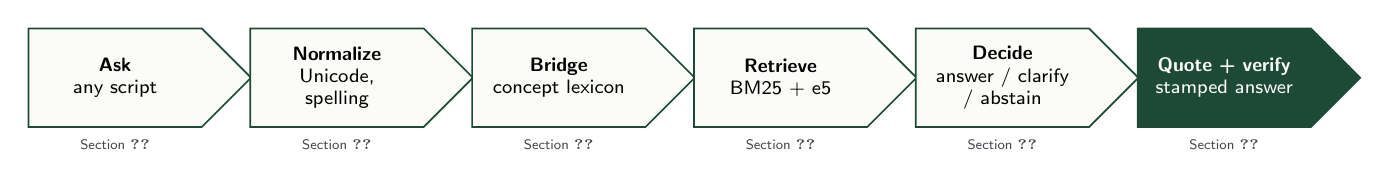
\begin{tikzpicture}[
  stg/.style={signal, signal to=east, draw=esgreen, fill=essheet, line width=0.6pt, minimum height=1.25cm, text width=1.78cm,
               align=center, font=\sffamily\scriptsize, inner xsep=6pt},
  first/.style={stg, signal from=nowhere}]
  \node[first] (s1) {\textbf{Ask}\\ any script};
  \node[stg, right=-1pt of s1] (s2) {\textbf{Normalize}\\ Unicode, spelling};
  \node[stg, right=-1pt of s2] (s3) {\textbf{Bridge}\\ concept lexicon};
  \node[stg, right=-1pt of s3] (s4) {\textbf{Retrieve}\\ BM25 + e5};
  \node[stg, right=-1pt of s4] (s5) {\textbf{Decide}\\ answer / clarify / abstain};
  \node[stg, right=-1pt of s5, fill=esgreen, text=white] (s6) {\textbf{Quote + verify}\\ stamped answer};
  \foreach \n/\s in {s1/\ref{sec:arch}, s2/\ref{sec:norm}, s3/\ref{sec:lexicon}, s4/\ref{sec:retrieval}, s5/\ref{sec:decisions}, s6/\ref{sec:answer}}
    \node[below=1pt of \n, font=\sffamily\tiny\color{esink2}] {Section \s};
\end{tikzpicture}
\caption{The six stages every question passes through, and where each is explained in this report.}
\label{fig:roadmap}
\end{figure}

\textbf{What makes this system different from a chatbot.} It never writes its own answer. It finds the official sentence,
proves the quote is exact, and says so with a stamp. When no sentence supports an answer, it says ``not on record'' instead of
guessing. The table below shows the three possible outcomes; each has its own stamp in the interface (Section~\ref{sec:gui}).

\begin{table}[H]
\centering\small
\begin{tabularx}{\textwidth}{@{}l l X@{}}
\toprule
Stamp & Decision & Meaning for the citizen\\
\midrule
\stamp{esviolet}{Verified true copy} & \texttt{answer} & An exact quote from a DGI\&P page answers the question; the passage code and source link are shown.\\[4pt]
\stamp{esochre}{Particulars required} & \texttt{clarify} & The question could mean several services (e.g.\ ``how much does it cost?''); the user is asked which one.\\[4pt]
\stamp{esred}{Not on record} & \texttt{abstain} & The official passages don't support an answer, the question is out of scope, or the request is unsafe.\\
\bottomrule
\end{tabularx}
\caption{The three decisions and their stamps.}
\label{tab:stamps}
\end{table}

\tableofcontents
\newpage

% ================================================================== 1 introduction
\section{Introduction}
\label{sec:intro}

\subsection{The problem}
Pakistan's passport rules live on official web pages written mostly in English. Citizens ask about them in Urdu script, in
Roman Urdu (Urdu written in Latin letters, with no fixed spelling), in English, or in a mix of all three. The same question can
arrive in very different forms:

\begin{table}[H]
\centering\small
\begin{tabularx}{\textwidth}{@{}l X@{}}
\toprule
Style & The same question\\
\midrule
English & Which documents are required to renew a passport?\\
Urdu script & \ur{پاسپورٹ کی تجدید کے لیے کون سی دستاویزات درکار ہیں؟}\\
Roman Urdu & Passport renew karwanay ke liye kya documents chahiye?\\
Noisy Roman Urdu & pasport renu karwana hy\\
Code-mixed & Passport renewal ke liye online apply karna hota hai ya office jana hota hai?\\
\bottomrule
\end{tabularx}
\caption{One intent, five surface forms. Keyword search fails on most of them because the official text is English.}
\label{tab:forms}
\end{table}

Two failure modes make this hard. \textbf{Retrieval} breaks when the query's script or spelling differs from the source.
\textbf{Generation} is dangerous: a fluent chatbot can confidently invent a fee, a document or a processing time, and a
citizen may act on it.

\subsection{Goals}
The challenge brief asks for an assistant that (1) retrieves the correct official evidence regardless of script, spelling or
paraphrase, (2) answers only what that evidence supports, with a traceable citation, and (3) abstains or asks for
clarification when evidence is missing, all measured on a documented test set with no external API calls.

\subsection{Contributions}
\begin{itemize}
  \item A \textbf{cross-script concept lexicon} that maps English, Urdu and Roman Urdu surface forms to shared concepts, so an
        Urdu query can match English evidence (Section~\ref{sec:lexicon}).
  \item A comparison of \textbf{eleven retrieval configurations}: keyword, character n-gram, multilingual dense (e5) and hybrid,
        with the production choice made on development data only (Section~\ref{sec:retrieval}).
  \item A \textbf{decision cascade} of rule gates plus dev-tuned thresholds that returns \emph{answer}, \emph{clarify} or
        \emph{abstain} (Section~\ref{sec:decisions}).
  \item \textbf{Extractive answering with a citation verifier}: every displayed claim is a verbatim official quote whose ID,
        URL and numbers are checked (Section~\ref{sec:answer}).
  \item An optional \textbf{local LLM layer} (Qwen2.5 3B) that writes a short summary from the verified quotes only, with an
        automatic check for invented numbers (Section~\ref{sec:llm}).
  \item A \textbf{web application} designed around the ``attested copy'' metaphor, bilingual and right-to-left aware
        (Section~\ref{sec:gui}).
  \item An \textbf{honest evaluation}: a blind set frozen before the final fixes, bootstrap confidence intervals and a leakage
        audit (Sections~\ref{sec:protocol}--\ref{sec:errors}).
\end{itemize}

\subsection{How the brief's requirements are met}
\begin{table}[H]
\centering\small
\begin{tabularx}{\textwidth}{@{}l X l@{}}
\toprule
Requirement & How E-Sahulat meets it & Section\\
\midrule
FR-1 Multilingual input & Urdu script, Roman Urdu, English and code-mixed queries; script detected automatically & \ref{sec:norm}\\
FR-2 Normalization & NFKC, Arabic$\to$Urdu letters, digits, elongation, fuzzy spelling repair & \ref{sec:norm}\\
FR-3 Two+ retrievers compared & 11 configurations: BM25, char TF-IDF, e5 dense, hybrids, rerankers & \ref{sec:retrieval}, \ref{sec:results}\\
FR-4 Evidence-grounded answers & Verbatim quote with passage code, title and DGI\&P link & \ref{sec:answer}\\
FR-5 Unanswerable queries & ``Not on record'' abstention and ``particulars required'' clarification & \ref{sec:decisions}\\
FR-6 Traceability & Passage IDs, document IDs, URLs and text hashes kept end to end; decision trace in the UI & \ref{sec:data}, \ref{sec:gui}\\
FR-7 Evaluation & Recall@5, MRR@5, citation support, abstention, cross-script, latency, with $n$ and CIs & \ref{sec:protocol}, \ref{sec:results}\\
FR-8 Usability & Web app with language choice, evidence view, knowledge base and evaluation pages & \ref{sec:gui}\\
\bottomrule
\end{tabularx}
\caption{Functional requirements from the challenge brief.}
\end{table}

% ================================================================== 2 data
\section{Data and provenance}
\label{sec:data}

\subsection{The organisers' dataset}
The hackathon supplied one file, \texttt{Multilingual\_E-Sahulat\_AI\_Hackathon\_Dataset.docx}, holding 150 JSON records:
90 \texttt{train\_dev} records (30 intents \texttimes{} English, Urdu and Roman Urdu) and 60 \texttt{test} records (30 hard
cases \texttt{N001}--\texttt{N030} and 30 noisy Roman Urdu spelling variants \texttt{SV001}--\texttt{SV030}). Each answerable
record carries the official evidence excerpt in English and Urdu and its \texttt{dgip.gov.pk} source URL.

\subsection{The knowledge base}
The 30 distinct evidence excerpts (\texttt{F01}--\texttt{F30}) form the corpus. They come from 5 DGI\&P pages. Each passage keeps:

\begin{notebox}[Example passage record (F12)]
\small\ttfamily
pid: F12 \quad doc\_id: D2 \quad topic: minor\_validity \quad authority: official\\
url: https://dgip.gov.pk/passport/ordinary-passport.php\\
text: Children under 15 years of age will be issued Passport having 05 years validity only.\\
text\_ur: {\rmfamily\ur{15 سال سے کم عمر بچوں کو صرف پانچ سال کی میعاد والا پاسپورٹ جاری ہوگا۔}}\\
fact\_key: validity\_children\_under\_15 = 5 years \quad sha256: (16-hex prefix) \quad freshness: needs\_manual\_review
\end{notebox}

The \textbf{English excerpt is always the cited text}. The Urdu translation is indexed (so Urdu queries can match it) and
shown beside the quote, but it is the organisers' translation, not an official one.

\subsection{Query sets}
The official \texttt{train\_dev} split has no unanswerable questions, which makes it impossible to tune an abstention threshold.
\NDevTeam{} team-written development queries were therefore added (out-of-domain, other services, ambiguous, personal, noise,
prompt injection, unsafe, and confusable siblings), used \emph{only} for tuning. A separate blind set of \NBlind{} questions was
written and its hash frozen before the final round of fixes; it is the primary result.

\begin{figure}[H]
\centering
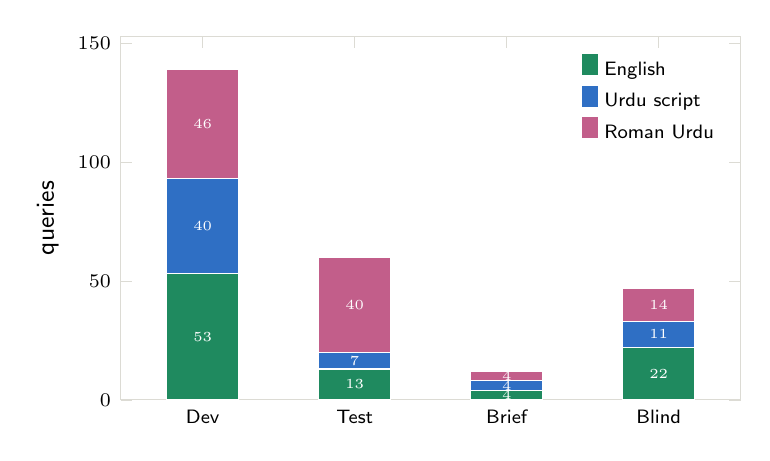
\begin{tikzpicture}
\begin{axis}[esaxis, ybar stacked, bar width=26pt, width=0.78\textwidth, height=6.2cm,
  symbolic x coords={Dev,Test,Brief,Blind}, xtick=data, ymin=0, ylabel={queries},
  legend style={at={(0.98,0.97)}, anchor=north east}, legend cell align=left,
  nodes near coords, every node near coord/.append style={font=\sffamily\tiny, color=white},
  enlarge x limits=0.18]
  \addplotcoords{fill=esseries, draw=white}{\SplitEn}
  \addplotcoords{fill=esblue, draw=white}{\SplitUr}
  \addplotcoords{fill=esrose, draw=white}{\SplitRoman}
  \legend{English, Urdu script, Roman Urdu}
\end{axis}
\end{tikzpicture}
\caption{Queries per split and language style ($\NQueriesAll$ in total). Dev = 90 official + \NDevTeam{} team-written; Test =
official \texttt{test} (60); Brief = the challenge's 12 validation cases; Blind = held-out set used once.}
\label{fig:splits}
\end{figure}

\begin{table}[H]
\centering\small
\begin{tabularx}{\textwidth}{@{}l l c X@{}}
\toprule
Split & Source & $n$ & Use\\
\midrule
Dev & official \texttt{train\_dev} + team queries & \NDev & Lexicon design, retriever selection, threshold tuning\\
Test & official \texttt{test} & \NTest & Seen during development, so used as a regression check only\\
Brief & the brief's 12 validation cases & \NBrief & Team-labelled; reported separately\\
Blind & written by the team, hashes frozen & \NBlind & Run once on the final pipeline; the honest measure\\
\bottomrule
\end{tabularx}
\caption{How each query set is used. The test split was never used for training or threshold tuning.}
\end{table}

% ================================================================== 3 architecture
\section{System architecture}
\label{sec:arch}

The system has three layers: a browser front end, a Python server that hosts the pipeline, and an optional local LLM.
Figure~\ref{fig:deploy} shows how they talk to each other; Figure~\ref{fig:pipeline} zooms into the pipeline.

\begin{figure}[H]
\centering
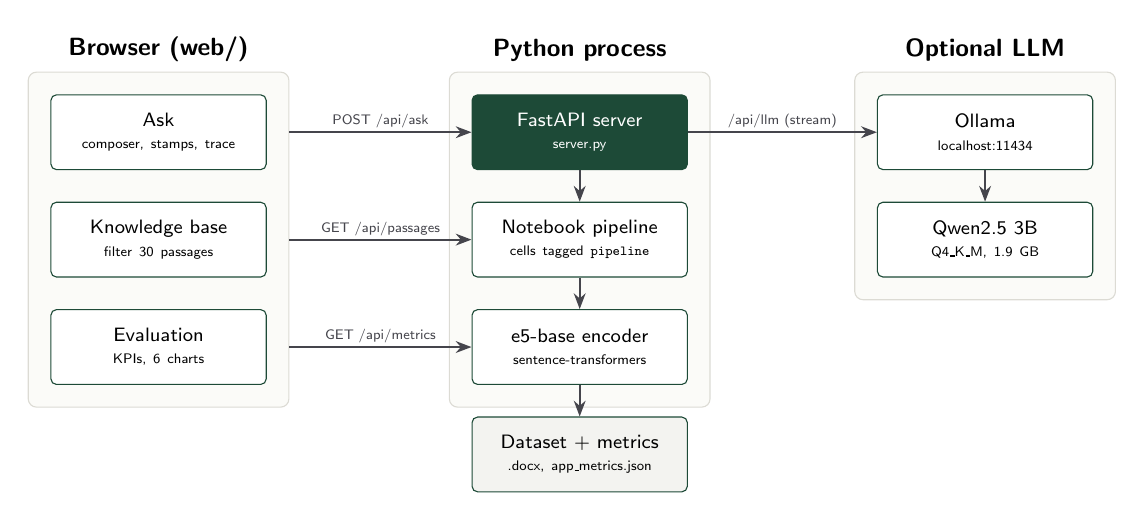
\begin{tikzpicture}[
  layer/.style={draw=esrule, fill=essheet, rounded corners=3pt, inner sep=8pt},
  comp/.style={draw=esgreen, fill=white, rounded corners=2pt, font=\sffamily\scriptsize, align=center, minimum height=0.95cm, text width=2.5cm},
  arr/.style={-{Stealth[length=2mm]}, thick, esink2},
  lab/.style={font=\sffamily\tiny, fill=white, inner sep=1pt}]
  \node[comp] (ui1) {Ask\\ \tiny composer, stamps, trace};
  \node[comp, below=4mm of ui1] (ui2) {Knowledge base\\ \tiny filter 30 passages};
  \node[comp, below=4mm of ui2] (ui3) {Evaluation\\ \tiny KPIs, 6 charts};

  \node[comp, right=2.6cm of ui1, fill=esgreen, text=white] (api) {FastAPI server\\ \tiny server.py};
  \node[comp, below=4mm of api] (pipe) {Notebook pipeline\\ \tiny cells tagged \texttt{pipeline}};
  \node[comp, below=4mm of pipe] (e5) {e5-base encoder\\ \tiny sentence-transformers};

  \node[comp, right=2.4cm of api] (ollama) {Ollama\\ \tiny localhost:11434};
  \node[comp, below=4mm of ollama] (qwen) {Qwen2.5 3B\\ \tiny Q4\_K\_M, 1.9 GB};

  \node[comp, below=4mm of e5, fill=espaper] (data) {Dataset + metrics\\ \tiny .docx, app\_metrics.json};
  \begin{scope}[on background layer]
    \node[layer, fit=(ui1)(ui2)(ui3), label={[font=\sffamily\small\bfseries]above:Browser (web/)}] (browser) {};
    \node[layer, fit=(api)(pipe)(e5), label={[font=\sffamily\small\bfseries]above:Python process}] (server) {};
    \node[layer, fit=(ollama)(qwen), label={[font=\sffamily\small\bfseries]above:Optional LLM}] (llm) {};
  \end{scope}

  \draw[arr] (browser.east |- ui1) -- node[lab, above] {POST /api/ask} (api.west);
  \draw[arr] (browser.east |- ui2) -- node[lab, above] {GET /api/passages} (pipe.west);
  \draw[arr] (browser.east |- ui3) -- node[lab, above] {GET /api/metrics} (e5.west);
  \draw[arr] (api) -- (pipe); \draw[arr] (pipe) -- (e5); \draw[arr] (e5) -- (data);
  \draw[arr] (api.east) -- node[lab, above] {/api/llm (stream)} (ollama.west);
  \draw[arr] (ollama) -- (qwen);
\end{tikzpicture}
\caption{Deployment. The server loads the notebook's pipeline cells at start-up, so the app runs exactly the evaluated code.
Nothing leaves the machine: Ollama and the e5 model both run locally.}
\label{fig:deploy}
\end{figure}

\begin{figure}[H]
\centering
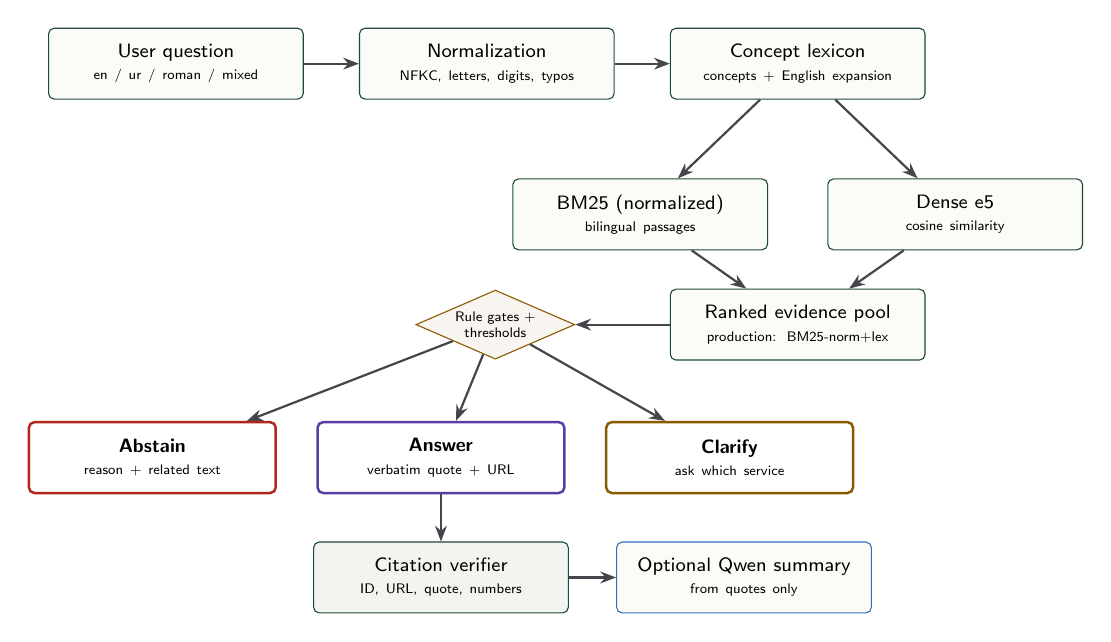
\begin{tikzpicture}[
  node distance=5mm and 7mm,
  box/.style={draw=esgreen, rounded corners=2pt, align=center, font=\sffamily\scriptsize, minimum height=9mm, text width=3.0cm, fill=essheet},
  gate/.style={draw=esochre, diamond, aspect=2.3, align=center, font=\sffamily\tiny, inner sep=1pt, fill=esochre!6},
  outc/.style={draw, rounded corners=2pt, align=center, font=\sffamily\scriptsize, minimum height=9mm, text width=2.9cm, line width=0.9pt},
  arr/.style={-{Stealth[length=2mm]}, thick, esink2}]
  \node[box] (q) {User question\\ \tiny en / ur / roman / mixed};
  \node[box, right=of q] (n) {Normalization\\ \tiny NFKC, letters, digits, typos};
  \node[box, right=of n] (c) {Concept lexicon\\ \tiny concepts + English expansion};
  \node[box, below=10mm of c, xshift=-2.0cm] (bm) {BM25 (normalized)\\ \tiny bilingual passages};
  \node[box, below=10mm of c, xshift=2.0cm] (de) {Dense e5\\ \tiny cosine similarity};
  \node[box, below=24mm of c] (rank) {Ranked evidence pool\\ \tiny production: \FinalMethod};
  \node[gate, left=12mm of rank] (g) {Rule gates +\\ thresholds};
  \node[outc, below left=10mm and -14mm of g, draw=esviolet] (a) {\textbf{Answer}\\ \tiny verbatim quote + URL};
  \node[outc, right=5mm of a, draw=esochre] (cl) {\textbf{Clarify}\\ \tiny ask which service};
  \node[outc, left=5mm of a, draw=esred] (ab) {\textbf{Abstain}\\ \tiny reason + related text};
  \node[box, below=6mm of a, fill=espaper] (v) {Citation verifier\\ \tiny ID, URL, quote, numbers};
  \node[box, right=6mm of v, draw=esblue] (l) {Optional Qwen summary\\ \tiny from quotes only};
  \draw[arr] (q) -- (n); \draw[arr] (n) -- (c);
  \draw[arr] (c) -- (bm); \draw[arr] (c) -- (de);
  \draw[arr] (bm) -- (rank); \draw[arr] (de) -- (rank);
  \draw[arr] (rank) -- (g);
  \draw[arr] (g) -- (a); \draw[arr] (g) -- (cl); \draw[arr] (g) -- (ab);
  \draw[arr] (a) -- (v); \draw[arr] (v) -- (l);
\end{tikzpicture}
\caption{The answering pipeline. The dense score feeds the decision thresholds even though the production \emph{ranking} is
keyword-based (Section~\ref{sec:retrieval}).}
\label{fig:pipeline}
\end{figure}

% ================================================================== 4 journey
\section{A question's journey, step by step}
\label{sec:journey}

To make the pipeline concrete, here is what actually happened to one Roman Urdu question in the running system
(pipeline \texttt{\PipelineVersion}). Every value below was read from the system's decision trace.

\begin{figure}[H]
\centering
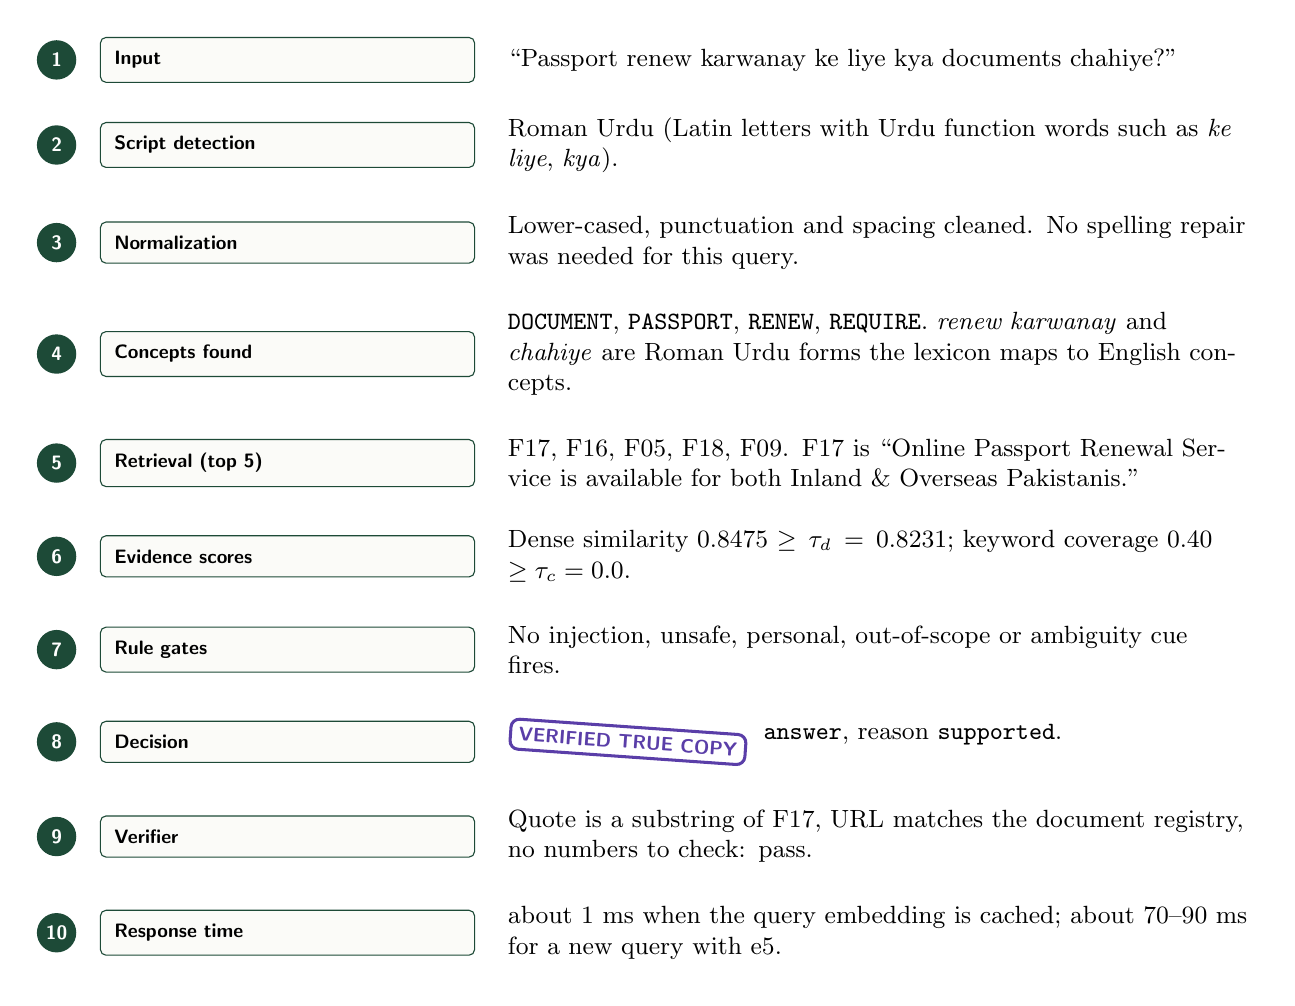
\begin{tikzpicture}[
  st/.style={draw=esgreen, fill=essheet, rounded corners=2pt, text width=4.4cm, font=\sffamily\scriptsize, inner sep=5pt, align=left},
  num/.style={circle, fill=esgreen, text=white, font=\sffamily\bfseries\scriptsize, inner sep=1.5pt, minimum size=5mm},
  val/.style={text width=9.4cm, font=\small, align=left, anchor=west},
  arr/.style={-{Stealth[length=2mm]}, thick, esrule}]
  \matrix[row sep=3.2mm, column sep=3mm] (m) {
    \node[num]{1}; & \node[st]{\textbf{Input}}; & \node[val]{``Passport renew karwanay ke liye kya documents chahiye?''}; \\
    \node[num]{2}; & \node[st]{\textbf{Script detection}}; & \node[val]{Roman Urdu (Latin letters with Urdu function words such as \emph{ke liye}, \emph{kya}).}; \\
    \node[num]{3}; & \node[st]{\textbf{Normalization}}; & \node[val]{Lower-cased, punctuation and spacing cleaned. No spelling repair was needed for this query.}; \\
    \node[num]{4}; & \node[st]{\textbf{Concepts found}}; & \node[val]{\texttt{DOCUMENT}, \texttt{PASSPORT}, \texttt{RENEW}, \texttt{REQUIRE}. \emph{renew karwanay} and \emph{chahiye} are Roman Urdu forms the lexicon maps to English concepts.}; \\
    \node[num]{5}; & \node[st]{\textbf{Retrieval (top 5)}}; & \node[val]{F17, F16, F05, F18, F09. F17 is ``Online Passport Renewal Service is available for both Inland \& Overseas Pakistanis.''}; \\
    \node[num]{6}; & \node[st]{\textbf{Evidence scores}}; & \node[val]{Dense similarity 0.8475 $\geq \tau_d=\TauDense$; keyword coverage 0.40 $\geq \tau_c=\TauCov$.}; \\
    \node[num]{7}; & \node[st]{\textbf{Rule gates}}; & \node[val]{No injection, unsafe, personal, out-of-scope or ambiguity cue fires.}; \\
    \node[num]{8}; & \node[st]{\textbf{Decision}}; & \node[val]{\stamp{esviolet}{Verified true copy}\; \texttt{answer}, reason \texttt{supported}.}; \\
    \node[num]{9}; & \node[st]{\textbf{Verifier}}; & \node[val]{Quote is a substring of F17, URL matches the document registry, no numbers to check: pass.}; \\
    \node[num]{10}; & \node[st]{\textbf{Response time}}; & \node[val]{about 1 ms when the query embedding is cached; about 70--90 ms for a new query with e5.}; \\
  };
\end{tikzpicture}
\caption{A real trace through the system. Steps 4 and 5 are where the cross-script bridge does its work: the query contains no
English word from F17 except ``passport'', yet F17 ranks first.}
\label{fig:journey}
\end{figure}

\begin{notebox}[The same intent in Urdu script]
The Urdu-script version, \ur{پاسپورٹ کی تجدید کے لیے کون سی دستاویزات درکار ہیں؟}, produced the same four concepts, the same
top-5 list (F17, F16, F05, F18, F09) and the same answer (F17), with dense similarity 0.8466. This is the cross-script
consistency the lexicon is designed for.
\end{notebox}

% ================================================================== 5 methods
\section{Methods}
\label{sec:methods}

\subsection{Query normalization}
\label{sec:norm}
Queries and passages go through the same meaning-preserving normalization, so both sides of the match look alike.

\begin{table}[H]
\centering\small
\begin{tabularx}{\textwidth}{@{}l X X@{}}
\toprule
Step & What it does & Example\\
\midrule
Unicode & NFKC, invisible characters removed & full-width or decomposed letters become standard\\
Letters & Arabic-keyboard \emph{yeh}, \emph{kaf}, \emph{heh} unified to Urdu code points & \ur{ي} $\to$ \ur{ی},\; \ur{ك} $\to$ \ur{ک}\\
Marks & diacritics and \emph{tatweel} removed; Urdu punctuation mapped & \ur{پاسپـــورٹ} $\to$ \ur{پاسپورٹ}\\
Digits & Urdu and Arabic-Indic digits to ASCII & \ur{۱۵} $\to$ 15\\
Roman Urdu & lower-case, letters repeated 3+ times collapsed, digit-letter split & \emph{10saal} $\to$ \emph{10 saal}, \emph{pleeease} $\to$ \emph{please}\\
Numbers & number words to digits & \emph{das}, \emph{ten} $\to$ 10\\
Spelling & fuzzy repair of unknown Latin tokens (below) & \emph{documnts} $\to$ \emph{documents}\\
\bottomrule
\end{tabularx}
\caption{Normalization steps.}
\end{table}

\textbf{Spelling-variant repair.} A Latin token $w$ of at least five characters that the lexicon does not know is replaced by the
closest known form, but only if it is close enough:
\begin{equation}
w^\ast = \arg\max_{v \in V_{\text{lex}}} \operatorname{sim}(w, v) \qquad \text{if} \quad \max_{v} \operatorname{sim}(w, v) \geq 0.84,
\end{equation}
where $\operatorname{sim}$ is the Ratcliff--Obershelp similarity ratio (Python's \texttt{difflib}). Known tokens are never
rewritten, and multi-word forms such as \emph{fst track} are matched as phrases.

\subsection{Cross-script concept lexicon}
\label{sec:lexicon}
More than fifty concepts list their English, Roman Urdu and Urdu-script surface forms. A query $q$ yields a concept set $C(q)$
and an expansion $E(q)$ of English terms taken from the corpus vocabulary; keyword retrievers then score $q \oplus E(q)$.

\begin{figure}[H]
\centering
\begin{tikzpicture}[
  form/.style={draw=esrule, fill=white, rounded corners=2pt, font=\small, minimum height=6.5mm, inner xsep=5pt},
  concept/.style={draw=esgreen, fill=esgreen, text=white, rounded corners=2pt, font=\sffamily\bfseries\small, minimum height=8mm, minimum width=2.4cm},
  exp/.style={draw=esblue, fill=esblue!6, rounded corners=2pt, font=\small, minimum height=6.5mm, inner xsep=5pt},
  arr/.style={-{Stealth[length=1.8mm]}, esink2}]
  \node[concept] (c) at (0,0) {RENEW};
  \node[form] (f1) at (-5.0, 1.4) {renew / renewal};
  \node[form] (f2) at (-5.0, 0.45) {renu / renew karwana};
  \node[form] (f3) at (-5.0,-0.5) {tajdeed};
  \node[form] (f4) at (-5.0,-1.45) {\ur{تجدید}};
  \node[font=\sffamily\tiny\color{esink2}] at (-5.0, 2.1) {surface forms (en / roman / ur)};
  \foreach \f in {f1,f2,f3,f4} \draw[arr] (\f.east) -- (c.west);
  \node[exp] (e1) at (4.6, 0.8) {renewal, renew};
  \node[exp] (e2) at (4.6,-0.2) {expiry, previous passport};
  \node[font=\sffamily\tiny\color{esink2}] at (4.6, 1.5) {English expansion terms};
  \draw[arr] (c.east) -- (e1.west); \draw[arr] (c.east) -- (e2.west);
\end{tikzpicture}
\caption{How one concept bridges scripts. Many surface forms map to \texttt{RENEW}, which adds English terms the official
passages actually use. Illustrative forms; the full lexicon is in the notebook (cell 8).}
\label{fig:lexicon}
\end{figure}

The lexicon also encodes \textbf{number phrases}, because several passages differ only by a number: ``\emph{N saal ka passport}''
means validity (F11/F12), while ``\emph{N saal ka bacha}'' means the applicant's age (F06/F07).

\subsection{Retrieval}
\label{sec:retrieval}
\textbf{Keyword retrieval (BM25).} Passages are scored with BM25Okapi ($k_1=1.5$, $b=0.75$):
\begin{equation}
\operatorname{BM25}(q, d) = \sum_{t \in q} \operatorname{IDF}(t)\cdot \frac{f(t,d)\,(k_1+1)}{f(t,d) + k_1\left(1 - b + b\,\frac{|d|}{\overline{|d|}}\right)},
\end{equation}
where $f(t,d)$ is how often token $t$ occurs in passage $d$ and $\overline{|d|}$ is the mean passage length.
\texttt{BM25-raw} uses raw text; \texttt{BM25-norm+lex} uses normalized text plus the lexicon expansion; the \texttt{+bi}
variants index the Urdu translation alongside the English passage.

\textbf{Character n-grams.} TF-IDF over character 3--5-grams (scikit-learn), a spelling-robust baseline.

\textbf{Dense retrieval.} The query and each passage are embedded with \texttt{\DenseModel} using the model's
\texttt{query:} and \texttt{passage:} prefixes and compared by cosine similarity:
\begin{equation}
s_{\text{dense}}(q, d) = \frac{\mathbf{e}_q \cdot \mathbf{e}_d}{\lVert \mathbf{e}_q \rVert\,\lVert \mathbf{e}_d \rVert}.
\end{equation}

\textbf{Hybrid fusion.} Rankings are fused with Reciprocal Rank Fusion, weighted by source authority $w_{a(d)}$ (1.0 official,
0.8 third-party):
\begin{equation}
s_{\text{RRF}}(d) = w_{a(d)} \sum_{r \in R} \frac{1}{60 + \operatorname{rank}_r(d)}.
\end{equation}

\textbf{Concept re-ranking.} The \texttt{+rerank} variants add $\lambda \cdot \operatorname{agree}(C(q), C(d))$ to separate
sibling passages that share most words (e.g.\ Normal / Urgent / Fast Track processing in F13--F15); $\lambda$ is tuned on dev.

\textbf{Selection.} All eleven configurations are run on dev, and the one with the best dev MRR@5 becomes the production
retriever. With e5 this was again \textbf{\FinalMethod}, which reached a perfect dev MRR@5 (Figure~\ref{fig:retdev}).

\subsection{Decision cascade}
\label{sec:decisions}
Each query gets exactly one decision through ordered gates. Rules handle the cases a similarity score can't (a prompt
injection can be highly similar to a real question); thresholds handle the rest.

\begin{figure}[H]
\centering
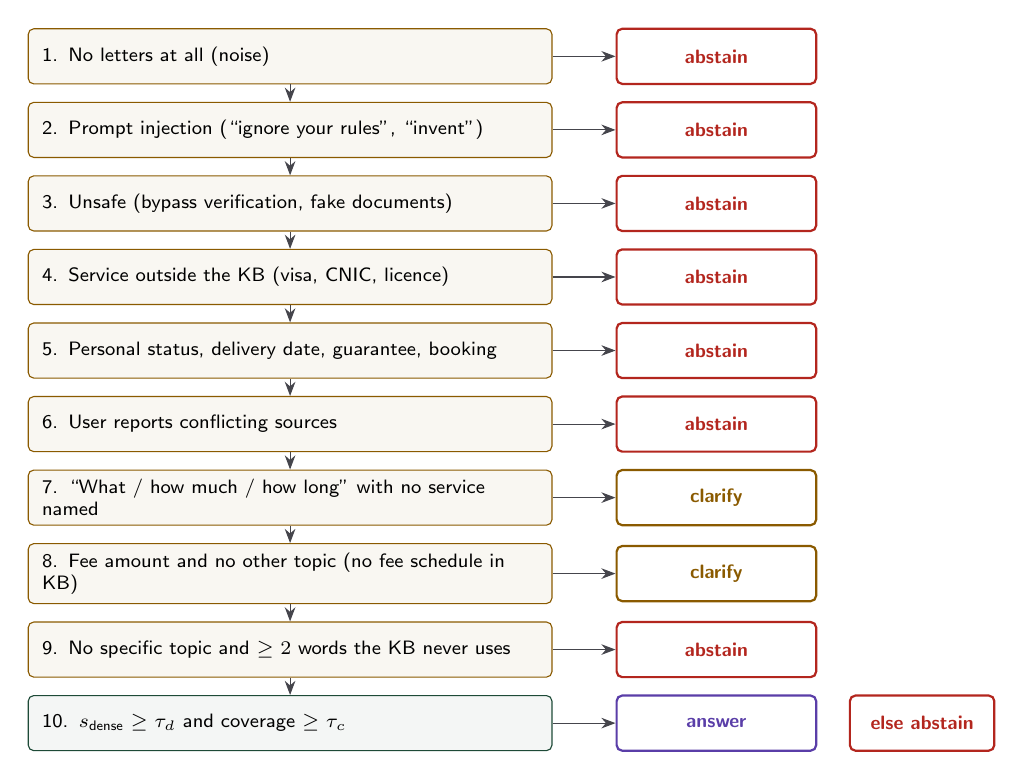
\begin{tikzpicture}[
  g/.style={draw=esochre, fill=esochre!5, rounded corners=2pt, font=\sffamily\scriptsize, text width=6.3cm, minimum height=7mm, align=left, inner xsep=5pt},
  o/.style={draw, rounded corners=2pt, font=\sffamily\scriptsize\bfseries, minimum height=7mm, text width=2.3cm, align=center, line width=0.8pt},
  arr/.style={-{Stealth[length=1.8mm]}, esink2}]
  \node[g] (g1) {1. No letters at all (noise)};
  \node[g, below=2.2mm of g1] (g2) {2. Prompt injection (``ignore your rules'', ``invent'')};
  \node[g, below=2.2mm of g2] (g3) {3. Unsafe (bypass verification, fake documents)};
  \node[g, below=2.2mm of g3] (g4) {4. Service outside the KB (visa, CNIC, licence)};
  \node[g, below=2.2mm of g4] (g5) {5. Personal status, delivery date, guarantee, booking};
  \node[g, below=2.2mm of g5] (g6) {6. User reports conflicting sources};
  \node[g, below=2.2mm of g6] (g7) {7. ``What / how much / how long'' with no service named};
  \node[g, below=2.2mm of g7] (g8) {8. Fee amount and no other topic (no fee schedule in KB)};
  \node[g, below=2.2mm of g8] (g9) {9. No specific topic and $\geq \TauUnknown$ words the KB never uses};
  \node[g, below=2.2mm of g9, draw=esgreen, fill=esgreen!5] (g10) {10. $s_{\text{dense}} \geq \tau_d$ and coverage $\geq \tau_c$};
  \foreach \i in {1,...,6,9} \node[o, draw=esred, text=esred, right=8mm of g\i] (o\i) {abstain};
  \foreach \i in {7,8} \node[o, draw=esochre, text=esochre, right=8mm of g\i] (o\i) {clarify};
  \node[o, draw=esviolet, text=esviolet, right=8mm of g10] (o10) {answer};
  \node[o, draw=esred, text=esred, right=4mm of o10, text width=1.6cm] (o11) {else abstain};
  \foreach \i in {1,...,10} \draw[arr] (g\i.east) -- (o\i.west);
  \foreach \i [evaluate=\i as \j using int(\i+1)] in {1,...,9} \draw[arr] (g\i.south) -- (g\j.north);
\end{tikzpicture}
\caption{The decision cascade. The first gate that fires decides; gate 10 is reached only by clean, in-domain questions.}
\label{fig:cascade}
\end{figure}

\textbf{Threshold tuning.} The thresholds are grid-searched on dev only, maximizing an objective that penalizes false answers
more than missed answers:
\begin{equation}
J(\tau) = 0.4\cdot \operatorname{Recall}_{\text{answer}}(\tau) + 0.6\cdot \operatorname{Acc}_{\text{non-answer}}(\tau),
\end{equation}
taking the middle of the best plateau for robustness. With e5 this gives $\tau_d=\TauDense$ and $\tau_c=\TauCov$.
Figure~\ref{fig:threshold} shows why a single cut can't be perfect: the two groups overlap.

\begin{figure}[H]
\centering
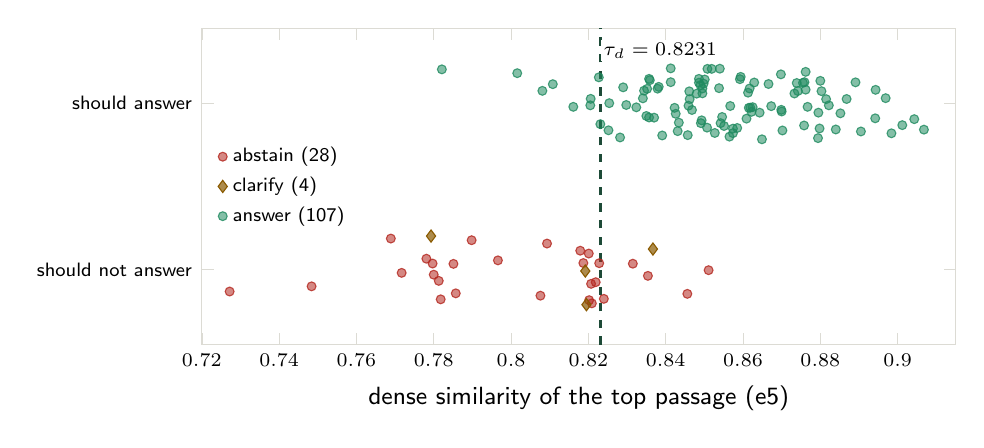
\begin{tikzpicture}
\begin{axis}[esaxis, width=0.92\textwidth, height=5.6cm, xmin=0.72, xmax=0.915, ymin=-0.45, ymax=1.45,
  ytick={0,1}, yticklabels={should not answer, should answer}, xlabel={dense similarity of the top passage (e5)},
  legend style={at={(0.01,0.5)}, anchor=west}, legend cell align=left]
  \addplotcoords{only marks, mark=*, mark size=1.6pt, color=esred, fill opacity=0.55, draw opacity=0.8}{\ThrAbs}
  \addplotcoords{only marks, mark=diamond*, mark size=2.2pt, color=esochre, fill opacity=0.7}{\ThrCla}
  \addplotcoords{only marks, mark=*, mark size=1.6pt, color=esseries, fill opacity=0.55, draw opacity=0.8}{\ThrAns}
  \draw[esgreen, very thick, dashed] (axis cs:\TauDense,-0.45) -- (axis cs:\TauDense,1.45);
  \node[font=\sffamily\scriptsize, fill=white, inner sep=1pt, anchor=south west] at (axis cs:\TauDense,1.25) {$\tau_d = \TauDense$};
  \legend{abstain (\ThrNAbs), clarify (\ThrNCla), answer (\ThrNAns)}
\end{axis}
\end{tikzpicture}
\caption{Dev questions by their top dense score, jittered vertically. Left of the dashed line the system abstains. \ThrAnsBelow{}
answerable questions fall below the threshold (missed answers) and \ThrNegAbove{} non-answerable ones sit above it; those are
caught by the rule gates or by low coverage instead.}
\label{fig:threshold}
\end{figure}

\subsection{Grounded answers and citation verification}
\label{sec:answer}
Answers are \textbf{extractive}: the top official passage is quoted word for word with its passage code, page title and URL.
Before anything is shown, a verifier checks every evidence item:
\begin{enumerate}[label=(\alph*)]
  \item the passage ID exists in the knowledge base;
  \item the URL equals the document registry entry for that passage;
  \item the quoted span is an exact substring of the passage;
  \item every number in the span appears in the passage.
\end{enumerate}
Tamper tests in the notebook (altered quote, wrong URL, unknown ID) confirm that the verifier rejects fabricated citations.
In the interface a failed check replaces the violet stamp with a red ``copy not verified'' stamp.

\textbf{Conflict handling.} Passages that state the same quantity share a \texttt{fact\_key}. If the evidence pool holds two
different values for one key, the response prefers the official (and, where dated, newer) source and discloses the
disagreement. The official KB has no contradictions, so this is demonstrated with a clearly labelled synthetic passage that is
never used in any metric.

\subsection{Optional local LLM summary}
\label{sec:llm}
Verbatim quotes are safe but can read stiffly. When the \emph{Qwen summary} switch is on, a local Qwen2.5 3B model rewrites the
already-verified quotes as one to three plain sentences. It is boxed in on every side:

\begin{figure}[H]
\centering
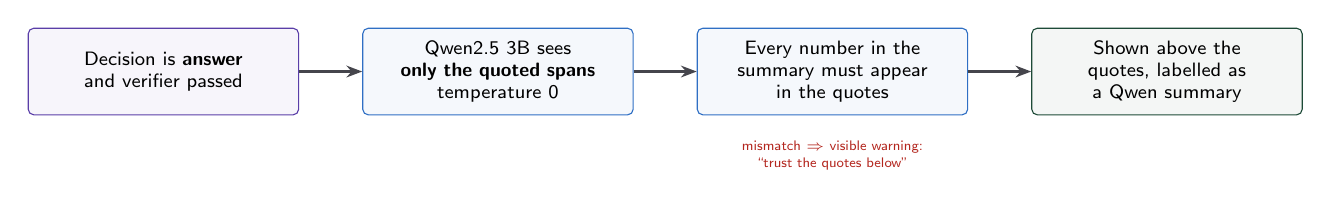
\begin{tikzpicture}[
  b/.style={draw=esblue, fill=esblue!5, rounded corners=2pt, font=\sffamily\scriptsize, text width=3.2cm, align=center, minimum height=1.1cm},
  arr/.style={-{Stealth[length=2mm]}, thick, esink2}]
  \node[b, draw=esviolet, fill=esviolet!5] (in) {Decision is \textbf{answer}\\ and verifier passed};
  \node[b, right=8mm of in] (llm) {Qwen2.5 3B sees\\ \textbf{only the quoted spans}\\ temperature 0};
  \node[b, right=8mm of llm] (chk) {Every number in the\\ summary must appear\\ in the quotes};
  \node[b, right=8mm of chk, draw=esgreen, fill=esgreen!5] (show) {Shown above the\\ quotes, labelled as\\ a Qwen summary};
  \draw[arr] (in) -- (llm); \draw[arr] (llm) -- (chk); \draw[arr] (chk) -- (show);
  \node[below=2mm of chk, font=\sffamily\tiny, text=esred, text width=3.4cm, align=center] {mismatch $\Rightarrow$ visible warning:\\ ``trust the quotes below''};
\end{tikzpicture}
\caption{Guardrails around the LLM. It runs only after the pipeline has already decided to answer, so it can never change a
decision, add a source, or answer a question the evidence doesn't support.}
\label{fig:llm}
\end{figure}

The system prompt instructs the model to keep every number, fee, document name and time period exactly as written, to mention
nothing not in the quotes, and to end each sentence with its passage ID. In testing, the summary for ``Can a child under 15 get a
ten-year passport?'' was: \emph{``No, children under 15 years of age will be issued Passport having 05 years validity only
[F12].''} The first summary after start-up took about 26\,s (model load); later ones took 8--17\,s on CPU.

% ================================================================== 6 models
\section{Models used}
\label{sec:models}

\begin{table}[H]
\centering\small
\begin{tabularx}{\textwidth}{@{}>{\bfseries}p{3.0cm} X X@{}}
\toprule
 & Dense encoder & Local LLM (optional)\\
\midrule
Model & \texttt{intfloat/multilingual-e5-base} & Qwen2.5 3B Instruct (\texttt{qwen2.5:3b})\\
Role & Embeds queries and passages; its similarity drives the answer/abstain threshold and the dense and hybrid retrievers & Rewrites verified quotes into a short plain-language summary\\
Architecture & XLM-RoBERTa encoder: 12 layers, 12 heads, 768-dim, 250k-token vocabulary & Qwen2 decoder, 3.1B parameters, 2048-dim embeddings, 32k context\\
Size on disk & about 1.1 GB (\textasciitilde 278M parameters) & 1.9 GB (Q4\_K\_M quantization)\\
Runtime & sentence-transformers 6.2 on PyTorch 2.14 (CPU) & Ollama, \texttt{localhost:11434}, temperature 0, at most 200 tokens\\
Languages & about 100, including Urdu & multilingual, including Urdu and English\\
Licence & MIT & Qwen Research License\\
Why chosen & Strong multilingual retrieval at a size that runs on a laptop CPU; no fine-tuning needed & Smallest capable instruction model that fits next to e5 in laptop memory\\
\bottomrule
\end{tabularx}
\caption{The two neural models. No model was trained from scratch; ``training'' here means tuning the retriever choice,
re-ranking weight and decision thresholds on the dev split.}
\label{tab:models}
\end{table}

\begin{notebox}[A note on the stand-in encoder]
An earlier round of the project could not download e5, so its numbers came from a character n-gram LSA stand-in
(\texttt{\StubVersion}). For this report the notebook was re-run end to end with the real e5 model (\texttt{\PipelineVersion});
every e5 number here comes from that run, and Section~\ref{sec:compare} compares the two.
\end{notebox}

\subsection{Software stack}
\begin{table}[H]
\centering\small
\begin{tabularx}{\textwidth}{@{}l X@{}}
\toprule
Layer & Technology\\
\midrule
Pipeline & Python 3.14, NumPy, pandas, scikit-learn, own BM25, \texttt{difflib}, \texttt{unicodedata}, python-docx\\
Neural & sentence-transformers + PyTorch (CPU) for e5; Ollama for Qwen\\
Server & FastAPI + Uvicorn (\texttt{server.py}): \texttt{/api/status}, \texttt{/api/ask}, \texttt{/api/passages}, \texttt{/api/metrics}, \texttt{/api/llm}, \texttt{/api/llm/start}\\
Front end & Hand-written HTML, CSS and JavaScript (no framework); SVG charts drawn from the metrics file\\
Evaluation & Bootstrap confidence intervals (2000 resamples), Matplotlib figures, generated \LaTeX{} tables\\
Report & \LaTeX{} (XeTeX via Tectonic), TikZ and pgfplots, figures generated from the run's outputs\\
\bottomrule
\end{tabularx}
\caption{Software used.}
\end{table}

% ================================================================== 7 gui
\section{The interface and its visual design}
\label{sec:gui}

\subsection{Design idea: the attested copy}
In Pakistan, an official document is trusted when it carries an attestation: a photocopy stamped and signed as a true copy.
The interface borrows that ritual. There is no chat thread. Each question produces one \emph{document}: the question as its
heading, a rubber stamp with the decision, and the official sentence laid on it as a paper strip cut from the source.

\begin{table}[H]
\centering\small
\begin{tabularx}{\textwidth}{@{}l X X@{}}
\toprule
Element & Visual treatment & Why\\
\midrule
Shell & bottle-green ``file cover'' top bar (\textcolor{esgreen}{\rule{8pt}{8pt}}~\#1D4A37) & reads as an official file, not a consumer app\\
Ground & cool photocopy white (\#F3F3F0) & paper without the warm ``cream'' cliché\\
Decisions & three stamp inks: violet, ochre, red & each outcome is recognizable at a glance; inks are reserved for decisions only\\
Quotes & serif text on a white strip with its own shadow & the official words look like an excerpt laid on file\\
Urdu & Nastaliq script, right to left, beside the English & every script is first-class, not a translation footnote\\
Passage codes & boxed green codes (F12) that link to the knowledge base & traceability with one click\\
Charts & green, blue and rose series, validated for colour-blind readers & chart colours never borrow a stamp ink\\
\bottomrule
\end{tabularx}
\caption{Visual vocabulary of the interface.}
\end{table}

\begin{figure}[H]
\centering
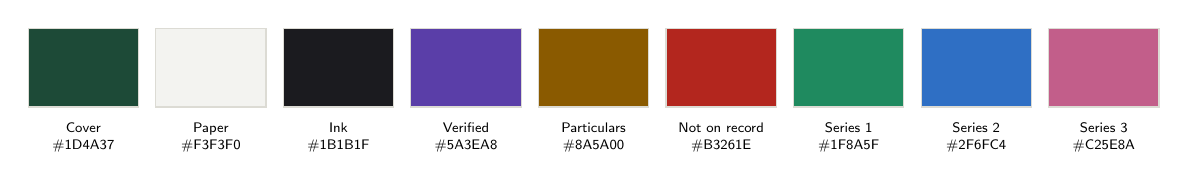
\begin{tikzpicture}
  \foreach \c/\n/\h [count=\i from 0] in {esgreen/Cover/1D4A37, espaper/Paper/F3F3F0, esink/Ink/1B1B1F, esviolet/Verified/5A3EA8, esochre/Particulars/8A5A00, esred/Not on record/B3261E, esseries/Series 1/1F8A5F, esblue/Series 2/2F6FC4, esrose/Series 3/C25E8A} {
    \fill[\c, draw=esrule] (\i*1.62, 0) rectangle ++(1.4, 1.0);
    \node[font=\sffamily\tiny, anchor=north, align=center] at (\i*1.62+0.7, -0.08) {\n\\ \#\h};
  }
\end{tikzpicture}
\caption{The palette. Stamp inks (violet, ochre, red) are used only for decisions; the chart series were checked with a
colour-vision-deficiency validator.}
\end{figure}

\subsection{Screens}
\begin{figure}[H]
\centering
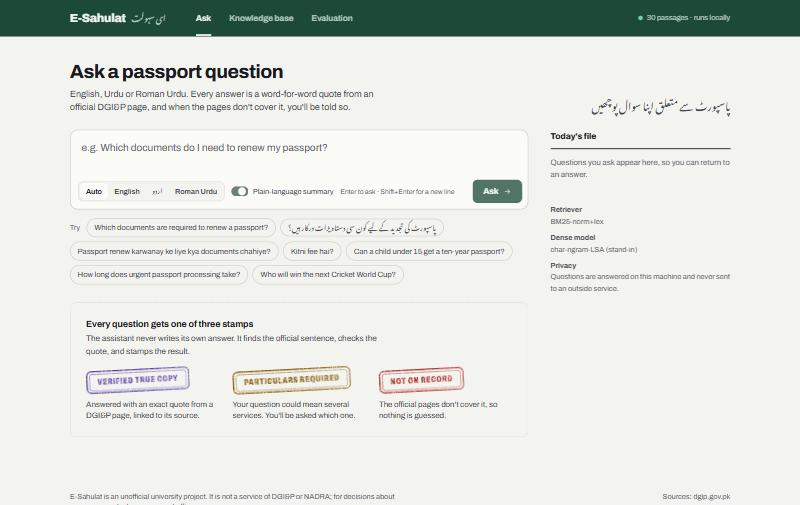
\includegraphics[width=0.92\textwidth]{figures/gui-empty.jpg}
\caption{First screen. The composer accepts any script (it switches to right-to-left when Urdu is typed). Below it, the three
stamps explain the possible outcomes before the first question; the right column keeps ``Today's file'' of asked questions.}
\label{fig:gui-empty}
\end{figure}

\begin{figure}[H]
\centering
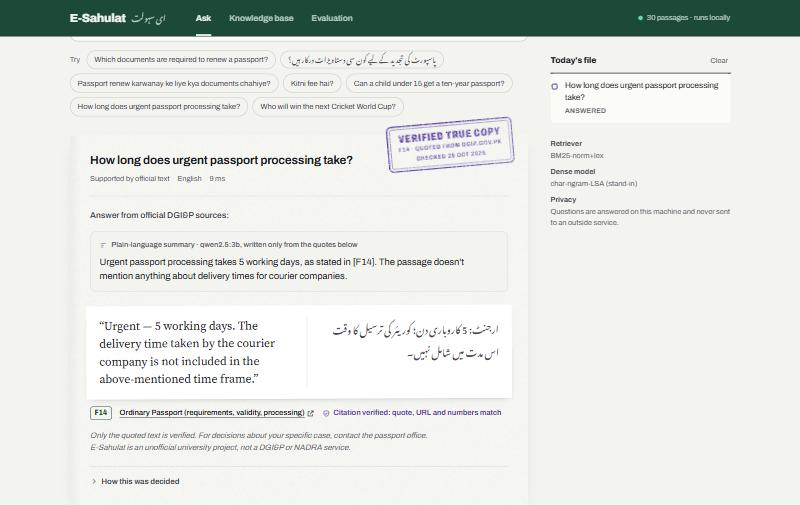
\includegraphics[width=0.92\textwidth]{figures/gui-answer.jpg}
\caption{An answered question. The violet stamp carries the passage code and check date. The Qwen summary sits above the
verbatim quote; the quote's Urdu text is mirrored across a centre rule; the source link and ``citation verified'' line follow.}
\label{fig:gui-answer}
\end{figure}

\begin{figure}[H]
\centering
\begin{subfigure}[t]{0.49\textwidth}\centering
  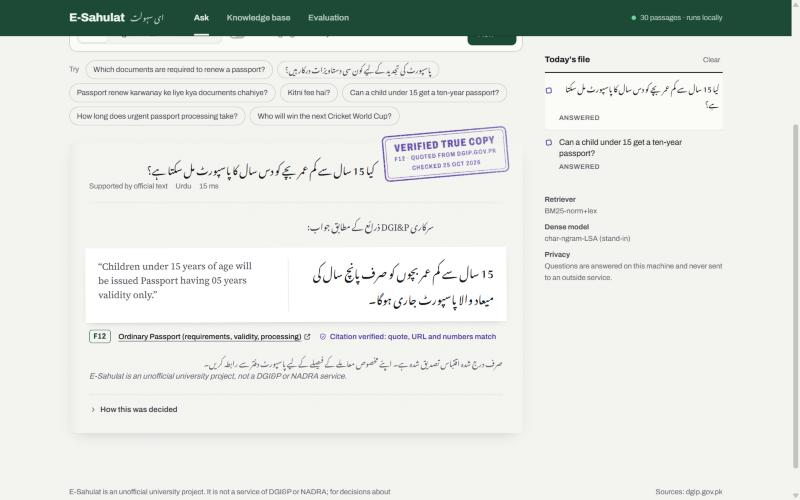
\includegraphics[width=\textwidth]{figures/gui-urdu.jpg}
  \caption{Urdu question: the Urdu text leads, on the right.}
\end{subfigure}\hfill
\begin{subfigure}[t]{0.49\textwidth}\centering
  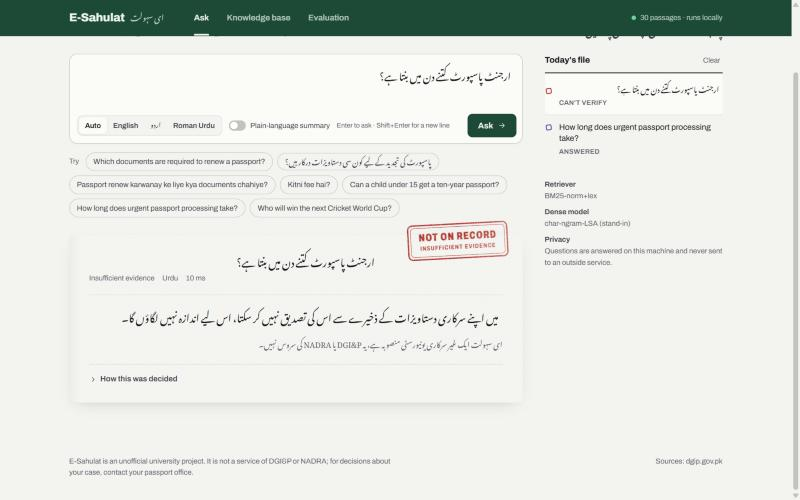
\includegraphics[width=\textwidth]{figures/gui-urdu-abstain.jpg}
  \caption{An unsupported Urdu question gets ``Not on record''.}
\end{subfigure}
\caption{Urdu is first-class: the layout mirrors for Urdu queries, and messages and disclaimers switch to Urdu.}
\end{figure}

\begin{figure}[H]
\centering
\begin{subfigure}[t]{0.49\textwidth}\centering
  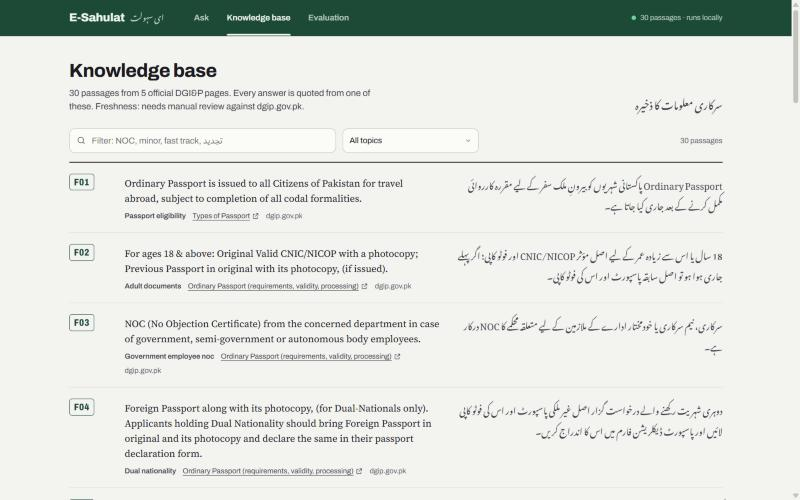
\includegraphics[width=\textwidth]{figures/gui-kb.jpg}
  \caption{Knowledge base: search and topic filter over the 30 passages.}
\end{subfigure}\hfill
\begin{subfigure}[t]{0.49\textwidth}\centering
  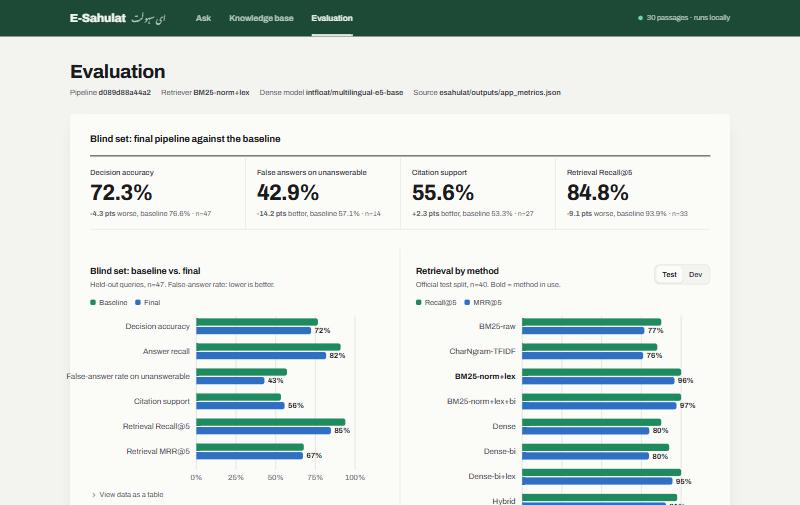
\includegraphics[width=\textwidth]{figures/gui-eval.jpg}
  \caption{Evaluation: blind-set KPIs against the baseline.}
\end{subfigure}
\caption{The two supporting sections. Every chart on the Evaluation page has a ``view data as a table'' alternative.}
\end{figure}

\begin{figure}[H]
\centering
\begin{subfigure}[b]{0.60\textwidth}\centering
  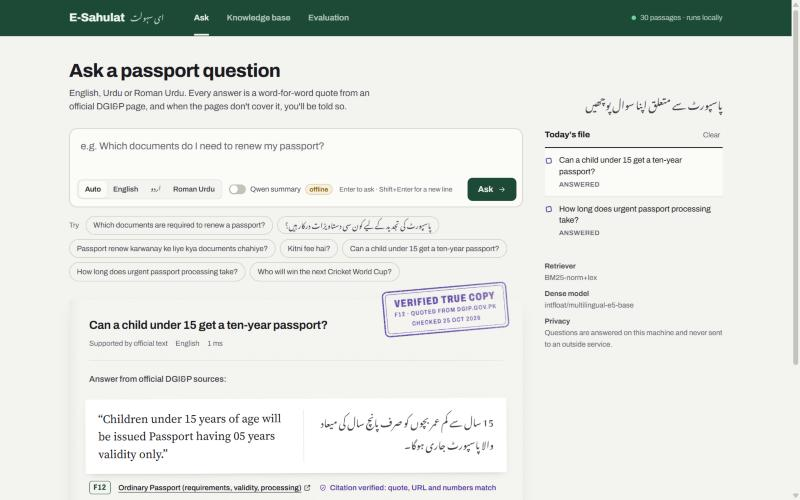
\includegraphics[width=\textwidth]{figures/gui-composer.jpg}
  \caption{Composer with the Qwen switch, here in its ``offline'' state.}
\end{subfigure}\hfill
\begin{subfigure}[b]{0.30\textwidth}\centering
  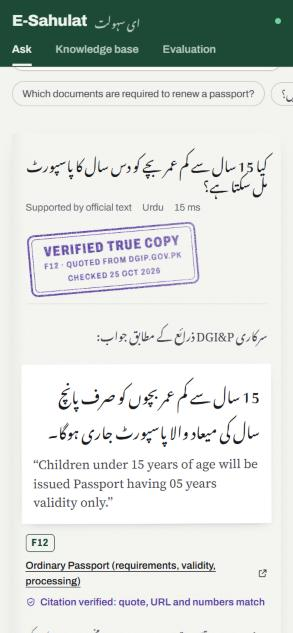
\includegraphics[width=\textwidth]{figures/gui-mobile-answer.jpg}
  \caption{Phone width (390\,px).}
\end{subfigure}
\caption{Controls and the phone layout. The Qwen switch shows the model's state (ready, starting, offline, model missing) and
starts Ollama when switched on.}
\end{figure}

\subsection{Interaction and accessibility}
\begin{itemize}
  \item \textbf{One signature motion.} The stamp lands on the document in 200\,ms with a strong ease-out curve; everything else
        uses short (\(\leq\)\,260\,ms) transitions on transform and opacity only, and all motion is reduced under the
        operating system's reduced-motion setting.
  \item \textbf{Honest states.} A loading banner while the pipeline boots, an empty state that teaches the three outcomes, a
        clear error when a request fails, and a visible state tag on the Qwen switch.
  \item \textbf{Accessibility.} WCAG AA contrast, full keyboard use, focus rings, \texttt{lang} and \texttt{dir} attributes on
        Urdu text, a table view behind every chart, and colour never used alone to carry meaning.
  \item \textbf{Responsible framing.} Every answer and the footer state that this is an unofficial university project, not a
        DGI\&P or NADRA service.
\end{itemize}

% ================================================================== 8 protocol
\section{Evaluation protocol}
\label{sec:protocol}

For answerable queries $Q_{\text{ans}}$ with gold passages $G_q$ and ranking $\pi_q$:
\begin{align}
\text{Recall@5} &= \frac{1}{|Q_{\text{ans}}|}\sum_{q} \mathbb{1}\!\left[G_q \cap \pi_q[1..5] \neq \emptyset\right], &
\text{MRR@5} &= \frac{1}{|Q_{\text{ans}}|}\sum_{q} \frac{1}{\operatorname{rank}_q}\quad\left(\tfrac{1}{\operatorname{rank}_q}=0 \text{ if } \operatorname{rank}_q>5\right).
\end{align}

\begin{itemize}
  \item \textbf{Decision accuracy}: share of queries whose decision (answer / clarify / abstain) matches the label.
  \item \textbf{False-answer rate}: share of unanswerable queries that were answered anyway. Lower is better; this is the
        metric that protects citizens.
  \item \textbf{Citation support}: share of answered queries whose citation passes the verifier \emph{and} points to a gold
        passage.
  \item \textbf{Cross-script consistency}: whether the English, Urdu and Roman Urdu versions of one intent retrieve the same top
        passage.
  \item \textbf{Latency}: end-to-end \texttt{respond()} time with the model loaded and per-query caches cleared.
\end{itemize}
Confidence intervals are 95\% percentile bootstraps over queries (2000 resamples). Because the official test queries were
visible during development, the \textbf{blind set is the primary result} and the official test is a regression check.

% ================================================================== 9 results
\section{Results}
\label{sec:results}

\subsection{Retrieval}
\begin{figure}[H]
\centering
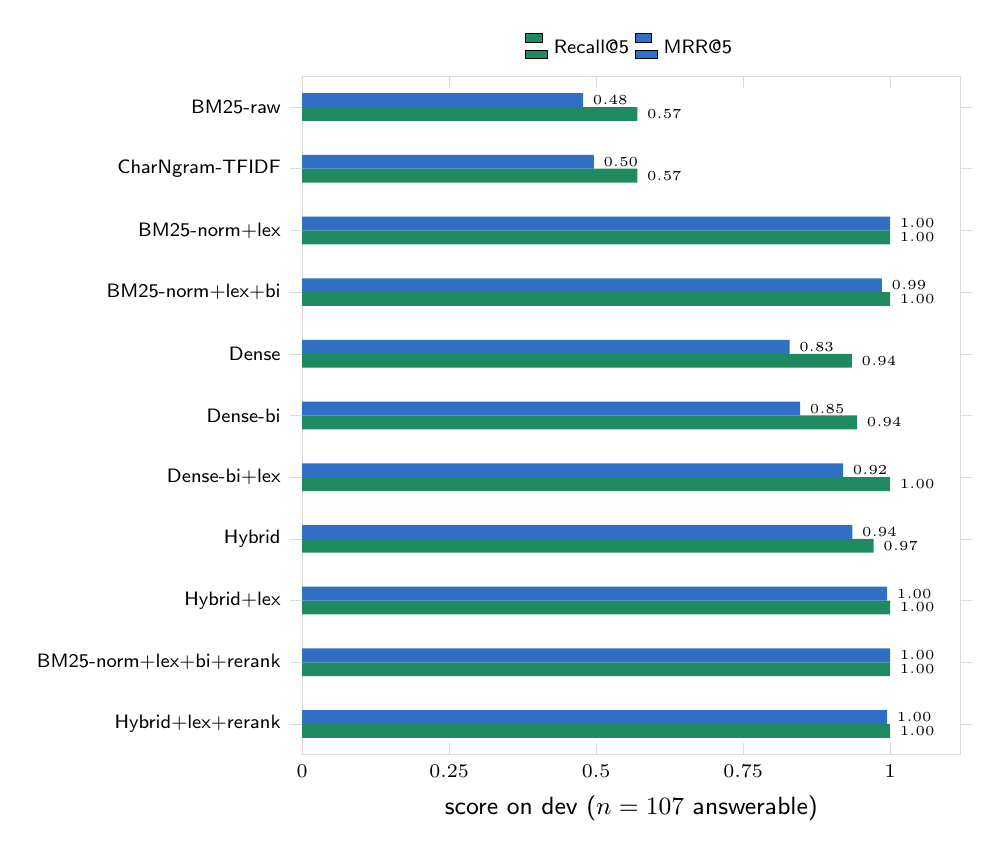
\begin{tikzpicture}
\begin{axis}[esaxis, xbar=0pt, bar width=5pt, width=0.82\textwidth, height=10.2cm, xmin=0, xmax=1.12,
  symbolic y coords/.expand once=\RetMethods, ytick=data, y dir=reverse, enlarge y limits=0.05,
  xlabel={score on dev ($n=\RetDevN$ answerable)}, xtick={0,0.25,0.5,0.75,1},
  legend style={at={(0.5,1.01)}, anchor=south, legend columns=2}, legend cell align=left,
  nodes near coords, nodes near coords align={horizontal}, every node near coord/.append style={font=\sffamily\tiny, /pgf/number format/.cd, fixed, fixed zerofill, precision=2}]
  \addplotcoords{fill=esseries, draw=none}{\RetDevRecall}
  \addplotcoords{fill=esblue, draw=none}{\RetDevMRR}
  \legend{Recall@5, MRR@5}
\end{axis}
\end{tikzpicture}
\caption{Retrieval on the development split, where the production retriever is chosen. Normalization plus the lexicon lifts
BM25 from 0.48 to 1.00 MRR@5; \FinalMethod{} is the first configuration to reach the top, so it was selected.}
\label{fig:retdev}
\end{figure}

\begin{figure}[H]
\centering
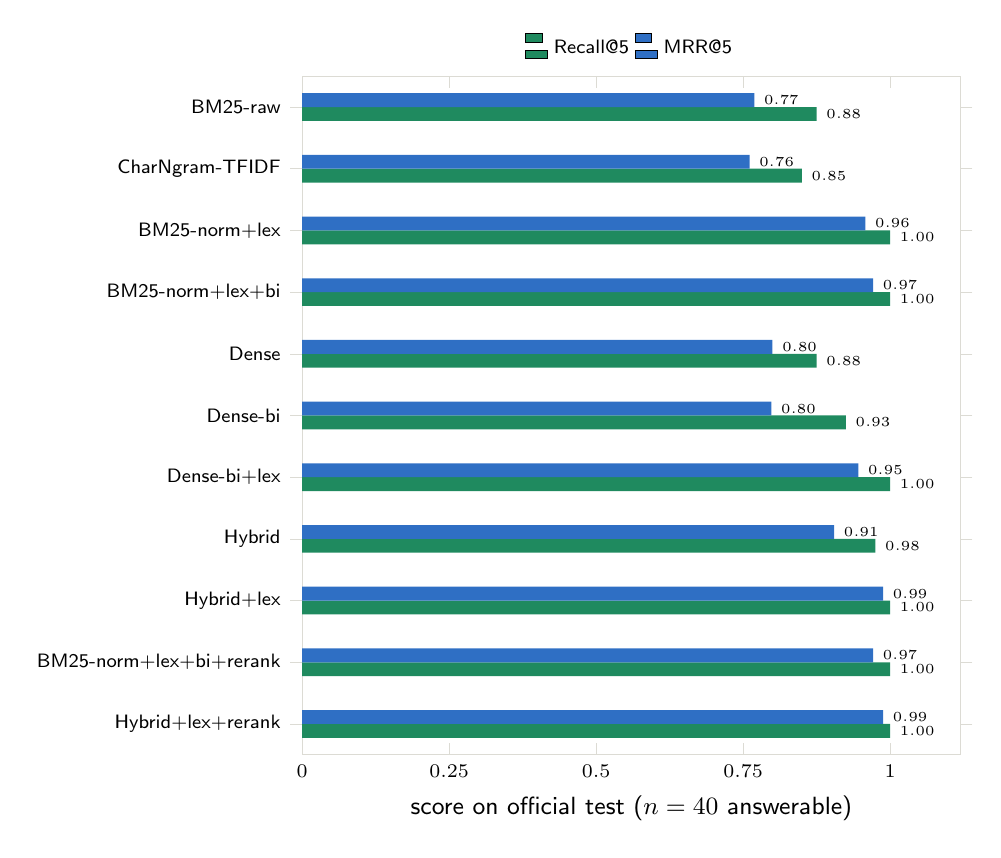
\begin{tikzpicture}
\begin{axis}[esaxis, xbar=0pt, bar width=5pt, width=0.82\textwidth, height=10.2cm, xmin=0, xmax=1.12,
  symbolic y coords/.expand once=\RetMethods, ytick=data, y dir=reverse, enlarge y limits=0.05,
  xlabel={score on official test ($n=\RetTestN$ answerable)}, xtick={0,0.25,0.5,0.75,1},
  legend style={at={(0.5,1.01)}, anchor=south, legend columns=2}, legend cell align=left,
  nodes near coords, nodes near coords align={horizontal}, every node near coord/.append style={font=\sffamily\tiny, /pgf/number format/.cd, fixed, fixed zerofill, precision=2}]
  \addplotcoords{fill=esseries, draw=none}{\RetTestRecall}
  \addplotcoords{fill=esblue, draw=none}{\RetTestMRR}
  \legend{Recall@5, MRR@5}
\end{axis}
\end{tikzpicture}
\caption{Retrieval on the official test split. The selected \FinalMethod{} reaches Recall@5 = \FinalRecall{} and MRR@5 =
\FinalMRR{} against \BaseRecall{} / \BaseMRR{} for raw BM25. Dense e5 alone reaches Recall@5 = \DenseRecall; combined with the
lexicon (\texttt{Hybrid+lex}) it reaches the highest test MRR@5, \HybridLexMRR, but that was not known when the choice was made
on dev.}
\label{fig:rettest}
\end{figure}

\subsection{Cross-script consistency}
For the 30 dev intents asked in all three scripts, the production retriever returns the same top passage in English, Urdu and
Roman Urdu for \CrossTopOne{} of intents, and all three hit the gold passage in their top 5 for \CrossAllHit. For the 30 noisy Roman
Urdu test variants, the top passage equals the English dev query's top passage \CrossSV{} of the time. Raw BM25 and character
n-grams score 0\% on the same-top-1 test, because Urdu script shares no tokens with English text.

\subsection{Blind set: the primary result}
\begin{figure}[H]
\centering
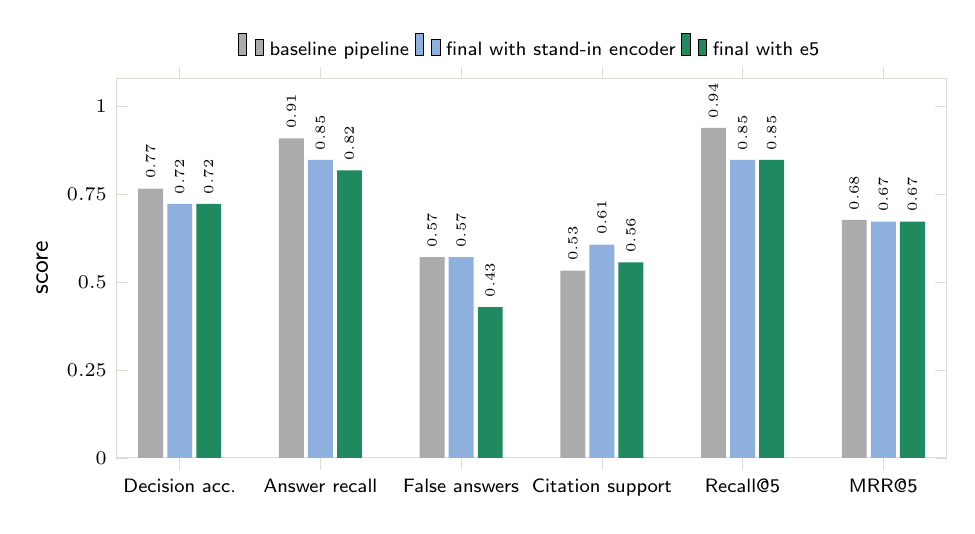
\begin{tikzpicture}
\begin{axis}[esaxis, ybar=1.5pt, bar width=9pt, width=\textwidth, height=6.4cm, ymin=0, ymax=1.08,
  symbolic x coords/.expand once=\BlindLabels, xtick=data, enlarge x limits=0.09, ylabel={score},
  ytick={0,0.25,0.5,0.75,1}, legend style={at={(0.5,1.02)}, anchor=south, legend columns=3}, legend cell align=left,
  nodes near coords, every node near coord/.append style={font=\sffamily\tiny, rotate=90, anchor=west, /pgf/number format/.cd, fixed, fixed zerofill, precision=2}]
  \addplotcoords{fill=esink2!45, draw=none}{\BlindBase}
  \addplotcoords{fill=esblue!55, draw=none}{\BlindStub}
  \addplotcoords{fill=esseries, draw=none}{\BlindEfive}
  \legend{baseline pipeline, final with stand-in encoder, final with e5}
\end{axis}
\end{tikzpicture}
\caption{Blind set ($n=\NBlind$; answerable $n=\BlindNRecall$, unanswerable $n=\BlindNFalse$). For ``false answers'' lower is
better. With e5, false answers drop from \BlindBaseFalse{} to \BlindEfiveFalse{} at the cost of answer recall
(\BlindBaseRecall{} $\to$ \BlindEfiveRecall). All confidence intervals overlap at this sample size.}
\label{fig:blind}
\end{figure}

\begin{table}[H]
\centering\small
\begin{tabular}{@{}lccc r@{}}
\toprule
Blind metric & Baseline & Stand-in final & \textbf{e5 final} & $n$\\
\midrule
Decision accuracy & \BlindBaseAcc & \BlindStubAcc & \textbf{\BlindEfiveAcc} & \BlindNAcc\\
Answer recall & \BlindBaseRecall & \BlindStubRecall & \textbf{\BlindEfiveRecall} & \BlindNRecall\\
False-answer rate (lower is better) & \BlindBaseFalse & \BlindStubFalse & \textbf{\BlindEfiveFalse} & \BlindNFalse\\
Citation support & \BlindBaseCite & \BlindStubCite & \textbf{\BlindEfiveCite} & \BlindNCite\\
Retrieval Recall@5 & \BlindBaseRecallFive & \BlindStubRecallFive & \textbf{\BlindEfiveRecallFive} & \BlindNRecallFive\\
Retrieval MRR@5 & \BlindBaseMRR & \BlindStubMRR & \textbf{\BlindEfiveMRR} & \BlindNMRR\\
Cross-language: all variants correct & \BlindBaseCross & \BlindStubCross & \textbf{\BlindEfiveCross} & \BlindNCross{} groups\\
\bottomrule
\end{tabular}
\caption{Blind results as numbers. The baseline is the pipeline before round-2 fixes.}
\end{table}

\subsection{Decisions across splits}
\begin{figure}[H]
\centering
\begin{minipage}[t]{0.52\textwidth}\centering
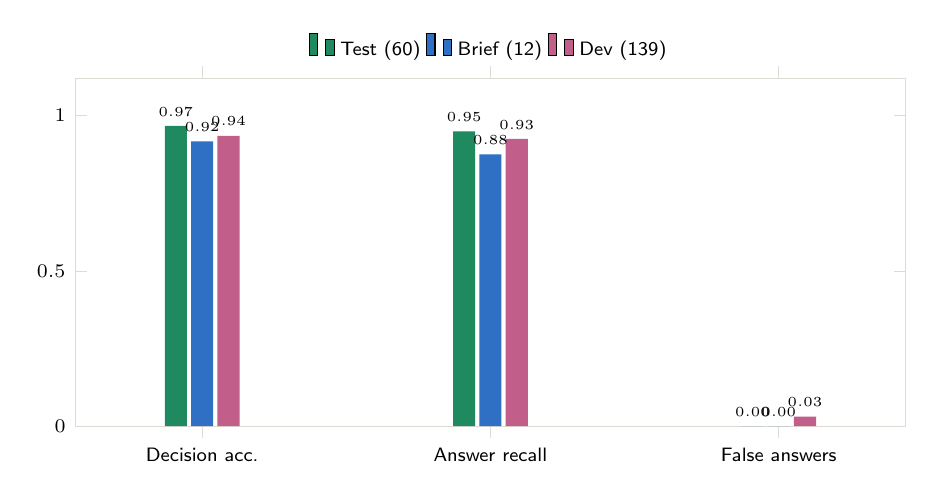
\begin{tikzpicture}
\begin{axis}[esaxis, ybar=1.5pt, bar width=8pt, width=\textwidth, height=6cm, ymin=0, ymax=1.12,
  symbolic x coords/.expand once=\DecLabels, xtick=data, enlarge x limits=0.22, ytick={0,0.5,1},
  legend style={at={(0.5,1.02)}, anchor=south, legend columns=3}, legend cell align=left,
  nodes near coords, every node near coord/.append style={font=\sffamily\tiny, /pgf/number format/.cd, fixed, fixed zerofill, precision=2}]
  \addplotcoords{fill=esseries, draw=none}{\DecTest}
  \addplotcoords{fill=esblue, draw=none}{\DecBrief}
  \addplotcoords{fill=esrose, draw=none}{\DecDev}
  \legend{Test (\DecTestN), Brief (\DecBriefN), Dev (\DecDevN)}
\end{axis}
\end{tikzpicture}
\end{minipage}\hfill
\begin{minipage}[t]{0.44\textwidth}\centering
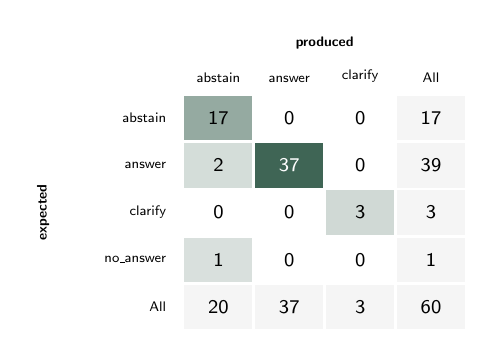
\begin{tikzpicture}[cmcell/.style={minimum width=0.9cm, minimum height=0.6cm, font=\sffamily\scriptsize, draw=white, line width=1pt}, x=0.9cm, y=0.6cm]
  \ConfCells
  \foreach \i/\n in \ConfRows \node[anchor=east, font=\sffamily\tiny] at (-0.6,-\i) {\n};
  \foreach \j/\n in \ConfCols \node[font=\sffamily\tiny, anchor=south] at (\j,0.55) {\n};
  \node[font=\sffamily\tiny\bfseries, anchor=south] at (1.5,1.25) {produced};
  \node[font=\sffamily\tiny\bfseries, rotate=90, anchor=south] at (-2.25,-2) {expected};
\end{tikzpicture}
\end{minipage}
\caption{Left: decision accuracy, answer recall and false-answer rate per split. Right: expected versus produced decisions on
the official test (darker = more queries). The one \texttt{no\_answer} query (an unsupported generalization) was correctly
not answered.}
\label{fig:decisions}
\end{figure}

On the official test the e5 pipeline makes the right decision for \TestAcc{} of queries, never answers an unanswerable one
(\TestFalse), and its citations are supported \TestCite{} of the time. On dev its false-answer rate is \DevFalse{}, down from
\StubDevFalse{} with the stand-in encoder.

\subsection{Latency}
\begin{figure}[H]
\centering
\begin{minipage}[b]{0.58\textwidth}\centering
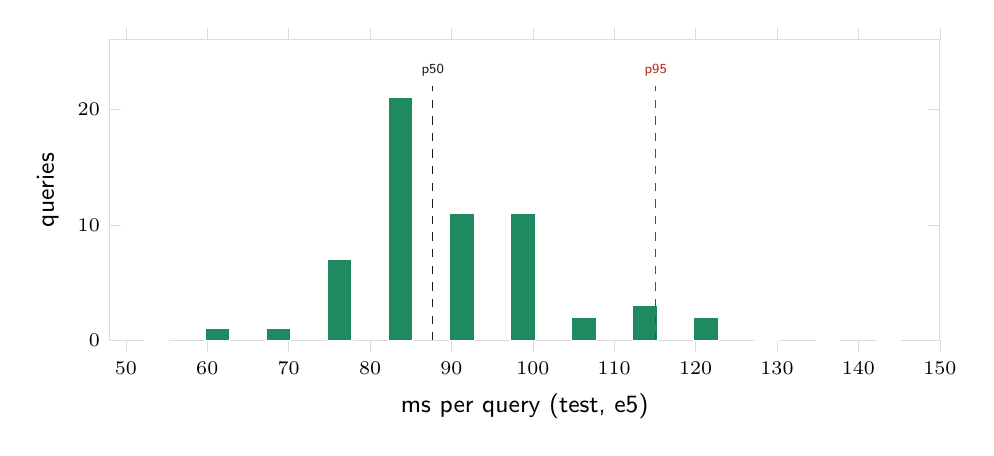
\begin{tikzpicture}
\begin{axis}[esaxis, ybar, bar width=9pt, width=\textwidth, height=5.4cm, ymin=0, xlabel={ms per query (test, e5)}, ylabel={queries},
  xmin=48, xmax=150, ymax=26]
  \addplotcoords{fill=esseries, draw=white}{\LatHist}
  \draw[esink, dashed] (axis cs:\LatEfivePfifty,0) -- (axis cs:\LatEfivePfifty,22) node[above, font=\sffamily\tiny] {p50};
  \draw[esred, dashed] (axis cs:\LatEfivePninetyfive,0) -- (axis cs:\LatEfivePninetyfive,22) node[above, font=\sffamily\tiny] {p95};
\end{axis}
\end{tikzpicture}
\end{minipage}\hfill
\begin{minipage}[b]{0.38\textwidth}\centering
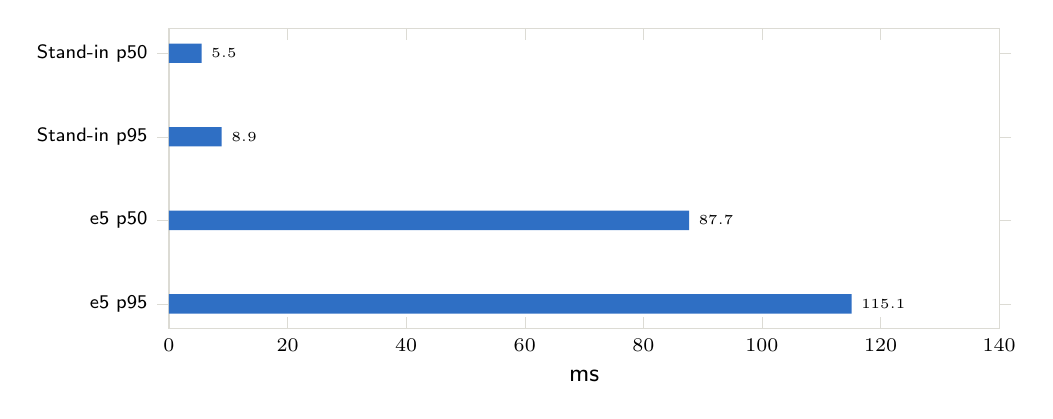
\begin{tikzpicture}
\begin{axis}[esaxis, xbar, bar width=7pt, width=\textwidth, height=5.4cm, xmin=0, xmax=140,
  symbolic y coords={Stand-in p50,Stand-in p95,e5 p50,e5 p95}, ytick=data, y dir=reverse, xlabel={ms},
  nodes near coords, every node near coord/.append style={font=\sffamily\tiny}]
  \addplot[fill=esblue, draw=none] coordinates {(\LatStubPfifty,Stand-in p50) (\LatStubPninetyfive,Stand-in p95) (\LatEfivePfifty,e5 p50) (\LatEfivePninetyfive,e5 p95)};
\end{axis}
\end{tikzpicture}
\end{minipage}
\caption{Response time on a laptop CPU (Intel Core i7-10510U). Embedding the query with e5 dominates: the median rises from \LatStubPfifty\,ms
(stand-in) to \LatEfivePfifty\,ms, still well below what a person notices. Repeated questions are cached and return in about 1\,ms.}
\label{fig:latency}
\end{figure}

% ================================================================== 10 errors
\section{Error analysis}
\label{sec:errors}

\begin{figure}[H]
\centering
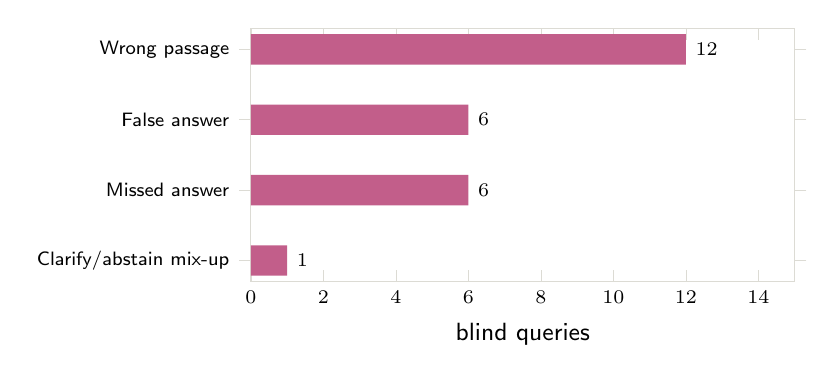
\begin{tikzpicture}
\begin{axis}[esaxis, xbar, bar width=11pt, width=0.7\textwidth, height=4.8cm, xmin=0, xmax=15,
  symbolic y coords/.expand once=\BlindErrLabels, ytick=data, y dir=reverse, xlabel={blind queries},
  nodes near coords, every node near coord/.append style={font=\sffamily\scriptsize}]
  \addplotcoords{fill=esrose, draw=none}{\BlindErr}
\end{axis}
\end{tikzpicture}
\caption{Error types on the blind set. ``Wrong passage'' means the decision was right (answer) but the cited passage was not the
gold one; it is the largest category.}
\label{fig:errors}
\end{figure}

\textbf{Official test and brief.} The e5 pipeline makes \TestErrors{} errors on the official test (\TestErrSibling{}
confusable-sibling citations and \TestErrMissed{} missed answers) and \BriefErrors{} on the brief's cases:

\begin{table}[H]
\centering\small
\begin{tabularx}{\textwidth}{@{}l X l l X@{}}
\toprule
ID & Query & Gold & Got & Cause\\
\midrule
N023 & Kya 2 working days ka matlab passport ghar bhi 2 din mein aa jaye ga? & F15 & F13 & sibling: Normal vs.\ Fast Track timing\\
SV008 & Minor k pasport k liye dono parents ki ID chahye? & F08 & F07 & sibling: two minor-document passages\\
SV018 & Online renewal kis condition mein hoti hy? & F18 & F17 & sibling: online renewal vs.\ its eligibility\\
SV011 & MRP 5 ya 10 saal ka hota hy? & F11 & abstain & dense score below $\tau_d$\\
SV023 & Passport office mein interview hota hy? & F23 & abstain & dense score below $\tau_d$\\
BC04 & Which documents are required to renew a passport? & F02/16/17/18 & F26 & ``a passport'' fuzzy-matched to ``e passport''\\
BC07 & pasport renu karwana hy & F16/17/18 & abstain & dense 0.8169, just under $\tau_d=\TauDense$\\
\bottomrule
\end{tabularx}
\caption{Every error on the official test and the brief. All are safe failures (a wrong-but-official quote or an abstention); none
invents information.}
\label{tab:errors}
\end{table}

\textbf{Patterns.}
\begin{itemize}
  \item \textbf{Sibling passages} that differ by one word or number (F13/F14/F15, F07/F08, F17/F18) are the main retrieval
        failure. Concept re-ranking helps on dev but not enough on noisy Roman Urdu.
  \item \textbf{The e5 threshold is strict.} It cuts false answers but also abstains on some heavily misspelled questions,
        such as the brief's Case 5B. That is the trade the tuning objective chose (Figure~\ref{fig:threshold}).
  \item \textbf{A known bug.} The phrase-level fuzzy matcher reads ``a passport'' as ``e passport'' and adds the
        \texttt{EPASS} concept, which pulled the English renewal question (BC04) to F26. The fix (exact match on a phrase's
        first token) was found after the blind run, so applying it requires a fresh blind set.
  \item \textbf{Blind false answers} (6 of \BlindNFalse) come from topics the KB doesn't cover (contact details, travel rules,
        fees), an ambiguous question containing a topic word, and an injection phrased without the cue words.
\end{itemize}

\subsection{Leakage audit}
The lexicon and rule cues were written with the official test visible. Dropping the 19 lexicon forms that occur only in test
queries lowers test Recall@5 from 1.000 to 0.975; dropping the 29 test-only cue phrases lowers test decision accuracy from 96.7\%
to 88.3\% and raises the false-answer rate from 0.0\% to 14.3\%. These ablated figures are the conservative estimate for the
official test, and they are why the blind set is treated as the primary result.

% ================================================================== 11 compare
\section{Stand-in encoder versus e5}
\label{sec:compare}
\begin{table}[H]
\centering\small
\begin{tabular}{@{}lcc@{}}
\toprule
 & Stand-in (\texttt{\StubVersion}) & e5 (\texttt{\PipelineVersion})\\
\midrule
Dense threshold $\tau_d$ & \StubTauDense & \TauDense\\
Production retriever & BM25-norm+lex & BM25-norm+lex\\
Blind decision accuracy & \BlindStubAcc & \BlindEfiveAcc\\
Blind false-answer rate & \BlindStubFalse & \textbf{\BlindEfiveFalse}\\
Blind answer recall & \BlindStubRecall & \BlindEfiveRecall\\
Blind citation support & \BlindStubCite & \BlindEfiveCite\\
Dev false-answer rate & \StubDevFalse & \textbf{\DevFalse}\\
Official test decision accuracy & \StubTestAcc & \TestAcc\\
Median latency (test) & \LatStubPfifty\,ms & \LatEfivePfifty\,ms\\
\bottomrule
\end{tabular}
\caption{What the real encoder changed.}
\end{table}

With e5 the dense score separates answerable from unanswerable questions more cleanly, so the tuned threshold moves up and the
system becomes more cautious: fewer false answers (the metric that protects citizens), slightly fewer answers overall. Ranking
quality is unchanged because the production ranker is keyword-based; e5's main contribution is \emph{knowing when not to
answer}. The \texttt{Hybrid+lex} configuration, which fuses e5 with the lexicon, now scores highest on test MRR@5, which
suggests it as the candidate to select once a fresh blind set exists.

% ================================================================== 12 limitations
\section{Limitations and responsible deployment}
\begin{itemize}
  \item \textbf{Small corpus.} With 30 passages, retrieval resembles intent classification. Scaling to full DGI\&P pages needs
        chunking and re-evaluation.
  \item \textbf{Hand-built rules.} The lexicon and gates were written by the same person who wrote the blind set; an
        independent test set is the next step.
  \item \textbf{No fee schedule.} Fees aren't in the knowledge base, so fee questions get a clarification or an abstention,
        never a number.
  \item \textbf{Freshness.} Official procedures change; every passage is marked ``needs manual review'' and must be
        re-checked against the live pages before any real deployment.
  \item \textbf{Translation.} The Urdu text is the organisers' translation; the English official excerpt stays authoritative.
  \item \textbf{Hardware.} Measured on a 16\,GB laptop (Intel Core i7-10510U, CPU only). With the app, e5 and Qwen all
        loaded, the full evaluation run ran out of memory until Qwen was unloaded.
  \item \textbf{Not an official service.} The interface says so on every answer.
\end{itemize}

\section{Practical impact}
The assistant targets citizens who search in Roman Urdu or Urdu, including people with limited English, and gives them
official, citable answers instead of forum hearsay. Refusing to guess about fees, guarantees or individual cases reduces the
risk of misleading people about legal requirements. The architecture (normalize, bridge, retrieve, decide, verify) transfers to
CNIC, licensing or other e-Sahulat services by swapping the corpus and extending the lexicon.

\section{Future work}
\begin{enumerate}
  \item Write an independent blind set (by someone who hasn't seen the lexicon) and fix the ``a passport'' matcher bug against it.
  \item Re-select the retriever with e5 on a larger dev set; \texttt{Hybrid+lex} is the leading candidate.
  \item Add a passage-level check that the cited sentence states the specific claim asked about, to cut wrong-passage answers.
  \item Expand the knowledge base from the live DGI\&P pages through the notebook's review-and-approve ingestion step.
  \item Self-host the web fonts so the interface renders fully offline.
\end{enumerate}

\section{Conclusion}
E-Sahulat retrieves official passport evidence across Urdu script, Roman Urdu, English and code-mixed questions, answers only
with verbatim, verified quotes, and says ``not on record'' when the evidence runs out. With the real e5 encoder it reaches
\BlindEfiveAcc{} decision accuracy on a blind set while answering unanswerable questions \BlindEfiveFalse{} of the time, down
from \BlindBaseFalse. The numbers are modest at $n=\NBlind$, and the report shows every failure, but each claim can be checked
against the notebook run that produced it.

\appendix
\section{Reproducing everything}
\begin{notebox}[Commands]
\small\ttfamily
pip install -r requirements.txt\\
python esahulat/run/run\_notebook.py \quad \rmfamily\itshape (or run the notebook top to bottom)\ttfamily\upshape\\
python report/make\_report\_data.py\\
cd report \&\& tectonic technical\_report.tex\\
python server.py \quad \rmfamily\itshape then open http://127.0.0.1:8000\ttfamily\upshape\\
ollama pull qwen2.5:3b \quad \rmfamily\itshape optional, for the Qwen summary
\end{notebox}

\begin{table}[H]
\centering\small
\begin{tabularx}{\textwidth}{@{}l X@{}}
\toprule
File & Contents\\
\midrule
\texttt{E\_Sahulat\_AI\_Hackathon.ipynb} & the pipeline, tuning and evaluation (cells tagged \texttt{pipeline} are what the app runs)\\
\texttt{server.py}, \texttt{web/} & the web application\\
\texttt{llm.py} & Ollama client, guardrails, number check, start-up helper\\
\texttt{esahulat/outputs/} & per-query results, error analysis, blind results, \texttt{app\_metrics.json} (generated)\\
\texttt{FINAL\_EVALUATION\_REPORT.md} & the run's own summary of every metric\\
\texttt{report/make\_report\_data.py} & turns the outputs into this report's numbers and charts\\
\texttt{DESIGN.md}, \texttt{PRODUCT.md} & the interface's design system and product notes\\
\bottomrule
\end{tabularx}
\caption{Where everything lives.}
\end{table}

Dataset fingerprint: SHA-256 prefix \texttt{5e0e45bce102a95a}; blind set: \texttt{2d821119487a}; random seed 42.

\end{document}
